
\documentclass[a4paper,fleqn]{cas-dc}

\usepackage[T1]{fontenc}
\usepackage[utf8]{inputenc}
\usepackage[authoryear,longnamesfirst]{natbib}
\usepackage{amsmath,amssymb,amsthm,mathtools}
\usepackage{booktabs,array,multirow}
\usepackage{enumitem}
\usepackage{graphicx}
\graphicspath{{../results/}{figures/}{./}}
\usepackage{tikz}
\usetikzlibrary{arrows.meta,positioning,calc}
\usepackage{xcolor}
\usepackage{placeins}
\usepackage{float}
\hypersetup{colorlinks=true,linkcolor=blue,citecolor=blue,urlcolor=blue,hypertexnames=false}
\emergencystretch=2em

\newtheorem{definition}{Definition}[section]
\newtheorem{theorem}[definition]{Theorem}
\newtheorem{proposition}[definition]{Proposition}
\newtheorem{lemma}[definition]{Lemma}
\newtheorem{corollary}[definition]{Corollary}
\theoremstyle{remark}
\newtheorem{remark}[definition]{Remark}
\newtheorem{example}[definition]{Example}

\newcommand{\R}{\mathbb{R}}
\newcommand{\Class}{\mathsf{Class}}
\newcommand{\Iclass}{\mathsf{I}}
\newcommand{\Hclass}{\mathsf{H}}
\newcommand{\Mclass}{\mathsf{M}}
\newcommand{\Dclass}{\mathsf{D}}
\newcommand{\Bclass}{\partial}
\newcommand{\Prof}{\Sigma}
\newcommand{\sgn}{\operatorname{sgn}}
\newcommand{\id}{\operatorname{id}}
\newcommand{\BR}{\operatorname{BR}}
\newcommand{\NE}{\operatorname{NE}}
\newcommand{\argmax}{\operatorname{arg\,max}}
\newcommand{\traj}{\operatorname{Traj}}

\begin{document}
\let\WriteBookmarks\relax
\def\floatpagepagefraction{1}
\def\textpagefraction{.001}

\shorttitle{Transporting Benefit--Loss Classes Across Contexts}
\shortauthors{C. Ramirez Ovalle}

\title[mode=title]{Transporting Benefit--Loss Classes Across Contexts:
Invariance and Equilibrium in Finite Games}

\author[1]{Carlos Ramirez Ovalle}[orcid=0000-0002-4254-5610]
\cormark[1]
\ead{carlosovalle@javerianacali.edu.co}
\affiliation[1]{organization={Pontificia Universidad Javeriana Cali},
                 addressline={Calle 18 No. 118-250},
                 city={Cali},
                 country={Colombia}}
\cortext[1]{Corresponding author}

\begin{abstract}
Existing game-theoretic formalizations of Cipolla's benefit--loss plane mainly encode its four classes as population strategies, while social-context models allow context to transform utilities. We ask a different comparative question: when a common finite action structure is transported between contexts, which profile classifications and pure incentives survive? Context-specific actor/affected-side payoff maps label profiles as intelligent, hapless, malicious, or destructive. Within the opponent-contingent separable family, we prove that preserving both the complete class map and all pure best responses for every valuation is equivalent to applying strictly increasing transformations that fix zero. Thus affine payoff offsets that are harmless to pure incentives can change social classification. We also derive exact open-ball radii for class maps and complete pure-equilibrium sets. A finite-game configuration theorem shows that intelligent and malicious equilibria cannot share the actor's action; sharing the affected-side action forces indifference and a knife-edge, whereas robust coexistence requires profiles sharing neither action. Three synthetic benchmarks separate class, equilibrium, and dynamic robustness. Reproducible audits enumerate 390,625 square and 1,062,882 rectangular payoff-grid games and apply seeded continuous perturbations. The contribution is a comparative theory of Cipolla-style profile classification, not a claim that context-dependent utility is new or that the benchmarks are empirical estimates.
\end{abstract}

\begin{keywords}
benefit--loss classification \sep contextual games \sep strategic equivalence
\sep Nash equilibrium \sep robustness \sep welfare \sep social modeling
\end{keywords}

\maketitle

\section{Introduction}

Social actions are rarely evaluated in a vacuum. A public correction, a disciplinary warning, a strategic sacrifice, or a managerial order may have different meanings in a company, a classroom, or a sport team. The same abstract action may be perceived as efficient leadership in one context, humiliation in another, and tactical discipline in a third. This observation motivates the present paper: if an interaction is evaluated through gains and losses, then its classification should depend not only on its formal strategic shape, but also on the context in which the payoffs are assigned.

Cipolla's benefit--loss plane provides a compact representation of this idea \citep{Cipolla2011}. An action performed by an agent can be represented by a point $(x,y)\in\R^2$, where $x$ is the gain or loss for the acting agent and $y$ is the gain or loss for the affected agent or group. The four main sign regions are interpreted as intelligent $(+,+)$, hapless $(-,+)$, malicious $(+,-)$, and stupid or destructive $(-,-)$ interactions. In the formal model developed here we use the term \emph{destructive}, not as a psychological diagnosis, but as a relational class of interactions producing non-compensating harm. The object of study is not a person; it is a strategic profile under a contextual valuation.

Existing formalizations inspired by Cipolla have explored evolutionary games, imitation dynamics, spatial interaction, agent-based modeling, and biophysical interpretations \citep{Kuperman2020, Barcenas2020, Tettamanzi2014, PerissiBardi2021}. These works establish that Cipolla's plane can support nontrivial games and population dynamics. Separately, social context games keep the players and strategies of an underlying game while using a network and aggregation rule to transform utilities \citep{AshlagiKrystaTennenholtz2008}. We do not claim priority for either embedding payoffs in games or allowing context to modify utility. Our question concerns the comparative semantics that remains between the two:
\begin{quote}
What does it mean to transport the same action structure from one social context to another while preserving, or failing to preserve, the benefit--loss class, pure-equilibrium membership, and population-level consequences of its interactions?
\end{quote}

We address this question with a family of \emph{contextual benefit--loss games}. Each member consists of finite action sets, a context, and a valuation map assigning every profile a point in the benefit--loss plane. Different contexts may share the action structure while assigning different payoff vectors to corresponding profiles. The primitive is deliberately simple; the contribution is the comparative structure placed on the family: translations, class invariance, pure strategic invariance, and exact distances to their failure.

The paper is organized around the valuation map $V_C:A\times B\to\R^2$, which induces three connected structures: a benefit--loss class partition, a normal-form game, and population-level observables under a specified adaptation rule. The key issue is that these readings retain different information. Payoff offsets conditional on an opponent's action can be invisible to pure incentives while moving profiles across Cipolla's axes. Conversely, two contexts can share every class while differing strategically. A transport theory must therefore say explicitly which structure it preserves.

The paper makes three principal contributions.
\begin{enumerate}[label=(\roman*)]
    \item \textbf{Comparative contribution.} Cipolla's labels are attached to profiles rather than persons or population strategies. Context translations compare corresponding profiles, and the induced partition provides the object whose preservation or reclassification is studied.
    \item \textbf{Joint-invariance contribution.} We characterize exactly which opponent-contingent separable transformations preserve both Cipolla classes and pure best responses universally: strictly increasing maps that fix zero. The affine intersection permits positive rescaling but no offsets. We then derive exact radii preserving class maps and complete pure-Nash sets, and characterize the possible relative positions of intelligent and malicious equilibria.
    \item \textbf{Computational contribution.} Exhaustive square and rectangular enumeration, seeded payoff perturbations, and an exponential-replicator illustration challenge the formal claims and separate class, equilibrium, and dynamic robustness. They are computational audits of synthetic games, not empirical validation.
\end{enumerate}

After defining the contextual game, the paper states the joint-preservation, exact-radius, and equilibrium-configuration results before developing general translations, class sensitivity, and robustness. The benchmark and dynamic sections apply those results. Saturated feature matrices and weight-space calculations are reported separately in Appendix~\ref{sec:features} so that the main argument does not depend on an unidentified parameterization.

The benchmark examples use three domains: a business organization with boss--employee players, a classroom with teacher--student players, and a sport team with coach--team members. The examples are not empirical measurements. They are normalized benchmark valuations generated from interpretable action features and context-specific weights. They show both stable profiles and context-sensitive profiles. In particular, the same abstract strategic profile---public pressure received with engaged uptake---may be malicious in a business organization, destructive in a classroom, and intelligent in a sport team. A second profile---constructive guidance met with resistance---shows a different transition pattern, from destructive to hapless to destructive.

The paper is a framework paper with a closed formal-computational contribution. It neither claims empirical validation of the benchmark payoffs nor proposes a new general theory of context-dependent preference. Its narrower claim is that Cipolla's sign semantics and strategic incentives define distinct invariance problems, and that studying them jointly yields restrictions and robustness conclusions that neither layer supplies alone.

\section{Related work and positioning}

\subsection{Cipolla-inspired games and simulations}

Cipolla's essay introduced a two-dimensional benefit--loss representation of social action. The core insight is that an action may benefit the actor, harm the other, benefit both, harm both, or benefit the other at the actor's expense. This qualitative plane gives a natural bridge to game theory, since each interaction can be read as a payoff vector.

Several formal extensions have already appeared. Kuperman, B\'{a}rcenas and Kuperman proposed an evolutionary game inspired by Cipolla, extending classical cooperator--defector schemes by introducing additional strategies, including one associated with destructive behavior \citep{Kuperman2020}. B\'{a}rcenas, Kuperman and Kuperman later studied a related evolutionary model in which destructive behavior can be adopted with a probability that affects the stationary distribution of strategies \citep{Barcenas2020}. Mella proposed the Social Wheel as a didactic extension of Cipolla's test by adding a third dimension related to the agent's willingness to generate advantages for others \citep{Mella2017}. Perissi and Bardi proposed a biophysical interpretation, connecting Cipolla's ideas with predator--prey and resource-exploitation models \citep{PerissiBardi2021}. Agent-based modeling has also been used to test Cipolla-like laws in artificial populations \citep{Tettamanzi2014}.

The present paper differs from these lines in three respects. First, Cipolla's
classes label realized profiles rather than inherited player types or population
strategies. Second, a profile can change class when the same action structure is
valued in another context. Third, the formal target is comparative invariance:
which labels and incentives survive a translation. Population dynamics are
included only as a downstream illustration.

\subsection{Social context games and strategic equivalence}

Ashlagi, Krysta and Tennenholtz introduced social context games by combining an
underlying strategic-form game with a neighborhood graph and aggregation
functions; players and strategies remain fixed while perceived utilities are
computed from the base payoffs \citep{AshlagiKrystaTennenholtz2008}. Subsequent
work studies equilibrium and inefficiency for particular graph and aggregation
families. This provides a direct precedent for context-sensitive utility in a
fixed strategic environment. Our context is not a graph-aggregation mechanism,
and no context is treated as the context-free base game. Instead, the family
$\{V_C\}$ is the primitive and the object transported is the Cipolla class map
induced on profiles.

A second adjacent literature studies when payoff transformations produce
strategically equivalent games. Tewolde and Conitzer characterize universal
preservation of Nash equilibria and best-response sets within broad separable
transformation families, highlighting positive affine transformations
\citep{TewoldeConitzer2024}. Strategic equivalence, however, is insensitive to
some payoff offsets, whereas benefit--loss classes depend on the location of
zero. Theorem~\ref{thm:joint-preservation} intersects the two requirements in
the opponent-contingent separable family. It shows precisely why the zero point
is substantive here: joint preservation requires strictly increasing maps that
fix zero, so shifts that preserve pure incentive order are excluded once
Cipolla's sign semantics must also be preserved.

\subsection{Mathematical social sciences, welfare, and formal social modeling}

The present paper is closest in spirit to the mathematical social sciences: it uses elementary formal structures to compare social meanings, payoff classifications, and strategic consequences across domains. We position it relative to four established literatures.

\paragraph{Social choice and welfare.} Comparing strategic profiles by their induced classes and by the aggregate $W=x+y$ is, at bottom, a question of how individual gains and losses are aggregated into a social judgment. The classical theory of social choice and welfare studies exactly such aggregations and their structural limits \citep{Arrow1951,Sen1970}, while utility and preference-representation theory clarifies when numerical payoffs can stand in for underlying preferences \citep{Fishburn1970}. Our $W$ is a deliberately minimal aggregate used only as a diagnostic, not as a contribution to welfare theory.

\paragraph{Payoff signs and strategic incentives.} The benefit--loss class of a profile depends only on the signs of its two payoff coordinates, whereas pure best responses depend on within-player payoff orderings \citep{vonNeumann1944,OsborneRubinstein1994}. Mixed equilibria and the population update used below also depend on payoff differences, so they are not invariant under arbitrary ordinal transformations. The framework therefore keeps three objects separate: payoff signs for class, unilateral comparisons for pure Nash equilibrium, and cardinal payoff gaps for mixed and dynamic analysis. The benchmarks belong to the long tradition of $2\times2$ interaction games \citep{Rapoport1965}; unlike games with vector payoffs, $(x,y)$ here is the ordinary pair of scalar payoffs to two players, not a multi-criterion payoff for one player.

\paragraph{Equilibrium robustness.} Stability and regularity of equilibrium components under game perturbations have an established technical meaning \citep{Jansen1981,KohlbergMertens1986}. We do not propose an equilibrium refinement or a notion of strategic stability in that sense. Theorem~\ref{thm:ne-radius} instead asks a narrower finite-game question: how large can a coordinate-wise payoff perturbation be while preserving the \emph{complete set of pure Nash profiles exactly}? For arbitrary finite two-player games the answer is an explicit radius in unilateral payoff slacks, which we compare with the independent radius preserving the benefit--loss class map.

\paragraph{Population and learning dynamics.} The dynamic layer places the same valuations inside a discrete exponential-replicator, or multiplicative-weights, process, connecting the framework to evolutionary learning and adaptive game play \citep{Weibull1995,HofbauerSigmund1998,FreundSchapire1999,Sandholm2010}. We use this layer only as a minimal aggregate illustration, not as an evolutionary or behavioral identification result.

\paragraph{Mathematical sociology and formal institutional models.} Finally, treating context as a formal component that fixes how actions are valued is consistent with the tradition of compact formal models in mathematical sociology and institutional analysis \citep{Gintis2009,Coleman1990,North1990,Ostrom2005}, where rules and roles determine the social meaning and consequences of behavior. In our terminology, an institution is encoded by a valuation map.

The local welfare function $W(x,y)=x+y$ used below is deliberately simple, but it allows the paper to separate two questions that are often conflated: whether a profile is a Nash equilibrium and whether it is socially desirable once both actor-side and affected-side payoffs are considered. This is important for the benchmark analysis, where one Nash equilibrium is malicious and welfare-dominated by another equilibrium.

\subsection{Behavioral and contextual game theory}

Behavioral game theory and decision theory have long emphasized that payoffs are not merely material outcomes. Framing, reference points, fairness, reciprocity, choice sets, and social preferences can alter evaluation of the same objective situation \citep{KahnemanTversky1979,TverskyKahneman1981,TverskySimonson1993,Rabin1993,FehrSchmidt1999}. The present model is consistent with that view but does not identify preferences from observed choice: the contextual valuation $V_C$ is an explicit model input. The paper provides a structural language for comparing consequences of alternative valuations, not a theory of how those valuations are formed.

Two recent contributions in \emph{Mathematical Social Sciences} sharpen this boundary. Su and Morsky add norm-derived relational utility to canonical games and study resulting changes in cooperation, coordination, and equilibria \citep{SuMorsky2024}. Ryan permits preferences in a stochastic-choice model to depend on the category through which alternatives are considered \citep{Ryan2026}. Our object is different from both: the strategy set and normal form are held fixed, context enters as an exogenously specified valuation map on profiles, and the analysis compares the induced sign partition with the exact pure-equilibrium set under payoff perturbations. We therefore neither derive context from a social-norm utility component nor estimate it from stochastic choice.

\subsection{Institutional analysis and social meaning}

Institutional analysis emphasizes that rules, roles, and collective goals shape the meaning and consequences of actions \citep{Ostrom2005}. A public correction has different institutional implications in a classroom, a firm, and a sport team because the relation between authority, performance, learning, discipline, and dignity differs across domains. In our terminology, institutional structure changes the valuation map. This is why the same strategic profile can be recontextualized without changing its abstract form.

\subsection{Positioning}

The paper therefore makes a deliberately narrower priority claim. It does not
introduce context-dependent utility, social-context games, or payoff
transformations. It develops a comparative theory for transporting
Cipolla-style benefit--loss labels across a family of finite games and for
separating preservation of those labels from preservation of incentives. The
framework links (i) profile-level class maps, (ii) context translations, (iii)
pure-equilibrium and welfare structure, and (iv) optional population dynamics.
This combination, rather than any one elementary definition, is the proposed
contribution.

\section{The benefit--loss plane as a partition}
\label{sec:plane}

Let $v=(x,y)\in\R^2$ be a payoff vector. The coordinate $x$ measures the payoff of the acting player, and $y$ measures the payoff of the affected player or group. Positive values represent gains, negative values represent losses, and zero values represent neutrality.

\begin{definition}[benefit--loss regions]
The benefit--loss regions of the benefit--loss plane are
\begin{align*}
\mathcal I &= \{(x,y)\in\R^2 : x>0,\ y>0\},\\
\mathcal H &= \{(x,y)\in\R^2 : x<0,\ y>0\},\\
\mathcal M &= \{(x,y)\in\R^2 : x>0,\ y<0\},\\
\mathcal D^- &= \{(x,y)\in\R^2 : x<0,\ y<0\},\\
\mathcal D^0 &= \{(x,y)\in\R^2 : x=0,\ y<0\}.
\end{align*}
The destructive region is
\[
\mathcal D = \mathcal D^-\cup \mathcal D^0.
\]
The boundary region is
\[
\partial\mathcal C = \R^2\setminus (\mathcal I\cup\mathcal H\cup\mathcal M\cup\mathcal D).
\]
\end{definition}

The class $\mathcal H$ is called \emph{hapless} rather than helpless in the sequel. It represents profiles in which the actor loses while the affected side gains. This terminology avoids suggesting a psychological incapacity and keeps the formal reading close to a payoff relation.

The inclusion of $\mathcal D^0$ in the destructive region (Figure~\ref{fig:plane-partition}) follows Cipolla's idea that an action may harm the other while producing no benefit for the actor. The strict region $\mathcal D^-$ represents mutual loss, while $\mathcal D^0$ represents non-compensating harm with actor-neutral payoff. We keep this distinction explicit because $\mathcal D^0$ lies on an axis and is therefore classifiable but structurally non-robust. This is a modeling convention rather than a mathematical necessity: one could instead put all zero-coordinate cases into the boundary, but doing so would lose the actor-neutral case of non-compensating harm that motivates $\mathcal D^0$. The main preservation, sensitivity, and robustness results are formulated so that alternative boundary conventions can be adopted with only local changes to the class map $Q$. In particular, all structural results below remain valid under alternative boundary conventions, after replacing $Q$ accordingly.

\begin{definition}[benefit--loss class map]
Let
\[
\Class=\{\Iclass,\Hclass,\Mclass,\Dclass,\Bclass\},
\]
where $\Iclass$ denotes intelligent, $\Hclass$ hapless, $\Mclass$ malicious, $\Dclass$ destructive, and $\Bclass$ boundary. The class map
\[
Q:\R^2\longrightarrow \Class
\]
is defined by
\[
Q(v)=
\begin{cases}
\Iclass, & v\in\mathcal I,\\
\Hclass, & v\in\mathcal H,\\
\Mclass, & v\in\mathcal M,\\
\Dclass, & v\in\mathcal D,\\
\Bclass, & v\in\partial\mathcal C.
\end{cases}
\]
\end{definition}

\begin{remark}[Actions rather than persons]
The formal model classifies strategic profiles or interactions, not persons. A person may participate in different contexts and may generate profiles with different classes. This distinction is essential for avoiding psychological essentialism and for making the model suitable for institutional and educational analysis.
\end{remark}

\begin{definition}[Local welfare]
The local welfare associated with a payoff vector $v=(x,y)$ is
\[
W(v)=x+y.
\]
\end{definition}

\begin{remark}[Welfare as a minimal diagnostic]
We use $W=x+y$ only as a minimal diagnostic aggregate, not as a full welfare theory. It assumes interpersonal comparability and linear aggregation of actor-side and affected-side payoffs. We adopt it solely to separate, in the benchmarks, whether a profile is a Nash equilibrium from whether it is socially desirable once both sides are counted; richer or non-linear social welfare functionals could replace it without affecting the class-level results.
\end{remark}

Under the stated convention every destructive profile has $W<0$.
Malicious profiles need not: $(5,-1)$ and $(1,-5)$ are both malicious,
but their local welfare has opposite signs.  Aggregate welfare can therefore
hide relational harm.  Points $(0,y)\in\mathcal D^0$ are classifiable but not
locally class-robust, since $(\delta,y)$ is malicious and $(-\delta,y)$ is
strictly destructive for every sufficiently small $\delta>0$.

\begin{figure*}[t]
\begin{center}
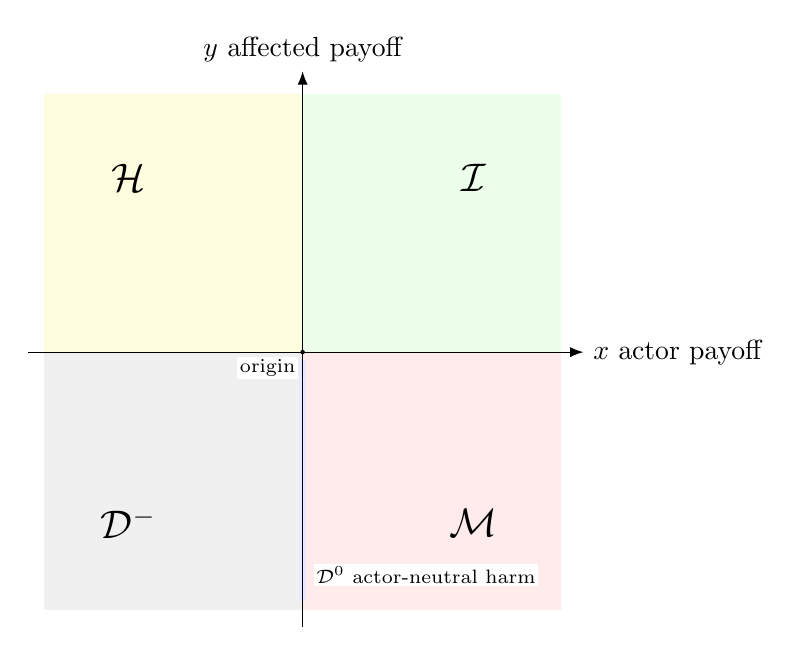
\begin{tikzpicture}[scale=0.82,>=Latex]
\fill[green!8] (0,0) rectangle (4.0,4.0);
\fill[yellow!12] (-4.0,0) rectangle (0,4.0);
\fill[red!8] (0,0) rectangle (4.0,-4.0);
\fill[gray!12] (-4.0,0) rectangle (0,-4.0);
\fill[blue!9] (-0.055,-3.85) rectangle (0.055,-0.12);
\draw[->] (-4.25,0) -- (4.35,0) node[right] {$x$ actor payoff};
\draw[->] (0,-4.25) -- (0,4.35) node[above] {$y$ affected payoff};
\fill[black] (0,0) circle (1.0pt);
\node[fill=white,inner sep=1pt,anchor=north east,font=\scriptsize] at (-0.06,-0.06) {origin};
\node[font=\Large] at (2.65,2.70) {$\mathcal I$};
\node[font=\Large] at (-2.70,2.70) {$\mathcal H$};
\node[font=\Large] at (2.65,-2.65) {$\mathcal M$};
\node[font=\Large] at (-2.70,-2.65) {$\mathcal D^{-}$};
\node[fill=white,inner sep=1pt,font=\scriptsize,anchor=west] at (0.16,-3.45) {$\mathcal D^0$ actor-neutral harm};
\end{tikzpicture}
\end{center}
\caption{\textbf{Benefit--loss partition.} Payoff space is divided into the intelligent region $\mathcal I$, the hapless region $\mathcal H$, the malicious region $\mathcal M$, and the destructive region $\mathcal D=\mathcal D^-\cup\mathcal D^0$. The thin vertical strip is the actor-neutral harmful set $\mathcal D^0$, included in $\mathcal D$ by modeling convention.}
\label{fig:plane-partition}
\end{figure*}

\begin{figure*}[t]
\begin{center}
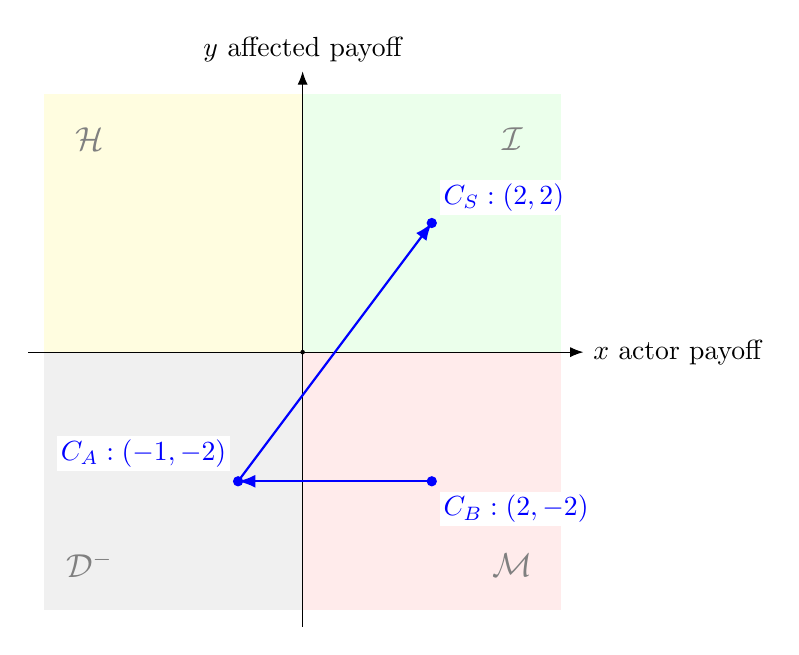
\begin{tikzpicture}[scale=0.82,>=Latex]
\fill[green!8] (0,0) rectangle (4.0,4.0);
\fill[yellow!12] (-4.0,0) rectangle (0,4.0);
\fill[red!8] (0,0) rectangle (4.0,-4.0);
\fill[gray!12] (-4.0,0) rectangle (0,-4.0);
\draw[->] (-4.25,0) -- (4.35,0) node[right] {$x$ actor payoff};
\draw[->] (0,-4.25) -- (0,4.35) node[above] {$y$ affected payoff};
\fill[black] (0,0) circle (1.0pt);
\node[font=\large,gray] at (3.25,3.30) {$\mathcal I$};
\node[font=\large,gray] at (-3.30,3.30) {$\mathcal H$};
\node[font=\large,gray] at (3.25,-3.30) {$\mathcal M$};
\node[font=\large,gray] at (-3.30,-3.30) {$\mathcal D^{-}$};
\draw[blue,thick,-{Latex[length=2.2mm]}] (2,-2) -- (-1,-2);
\draw[blue,thick,-{Latex[length=2.2mm]}] (-1,-2) -- (2,2);
\filldraw[blue] (2,-2) circle (2.0pt);
\filldraw[blue] (-1,-2) circle (2.0pt);
\filldraw[blue] (2,2) circle (2.0pt);
\node[blue,fill=white,inner sep=1.3pt,anchor=north west] at (2.12,-2.15) {$C_B:(2,-2)$};
\node[blue,fill=white,inner sep=1.3pt,anchor=south east] at (-1.12,-1.85) {$C_A:(-1,-2)$};
\node[blue,fill=white,inner sep=1.3pt,anchor=south west] at (2.12,2.12) {$C_S:(2,2)$};
\end{tikzpicture}
\end{center}
\caption{\textbf{Recontextualization of one profile.} The abstract profile $(P,U)$ is malicious in business $C_B$, destructive in classroom $C_A$, and intelligent in sport team $C_S$. The arrows represent contextual revaluation of the same strategic profile, not temporal motion.}
\label{fig:plane-recontext}
\end{figure*}

\section{Contextual benefit--loss games and induced partitions}
\label{sec:contextual-games}

An action structure alone does not determine a benefit--loss class. The class depends on how a context evaluates the consequences of the strategies. We therefore attach a valuation map to each context.

\begin{definition}[Contextual benefit--loss game]
A contextual benefit--loss game is a tuple
\[
G_C=(C,A,B,V_C),
\]
where $C$ is a context, $A$ is the strategy set of the acting or authority-side player, $B$ is the strategy set of the affected-side player, and
\[
V_C:A\times B\longrightarrow \R^2
\]
is a contextual valuation map. The profile set is denoted by
\[
\Prof_C=A\times B.
\]
For $\sigma\in\Prof_C$, the induced class is
\[
Q_C(\sigma)=Q(V_C(\sigma)).
\]
\end{definition}

A context may represent an organization, a classroom, a sport team, a family, a public institution, or any domain in which actions generate gains and losses for multiple agents. The context is not merely a label: it determines which consequences count as gains or losses and how they are normalized.

Write $V_C(a,b)=(X_C(a,b),Y_C(a,b))$.  The single valuation map
induces three structures:
\begin{enumerate}[label=(\roman*)]
\item A class map $Q_C=Q\circ V_C:A\times B\to \Class$ and hence a partition $\Pi_C$ of the profile set.
\item A two-player normal-form game with payoff functions $X_C:A\times B\to\R$ and $Y_C:A\times B\to\R$.
\item Once an adaptation rule $\mathcal L$ is fixed, a population update map on mixed strategy states; in the exponential-replicator case of Section~\ref{sec:simulation}, this is a map $(p_t,q_t)\mapsto(p_{t+1},q_{t+1})$.
\end{enumerate}
The first two are coordinate-wise readings of $V_C$; the third additionally
depends on the selected update rule.  They are not separate payoff inputs.

\begin{definition}[Induced benefit--loss partition]
Let $G_C=(C,A,B,V_C)$ be a contextual benefit--loss game. For each class $c\in\Class$, define
\[
\Prof_C^c=Q_C^{-1}(c)=\{\sigma\in A\times B:Q_C(\sigma)=c\}.
\]
The induced benefit--loss partition of $\Prof_C$ is
\[
\Pi_C=\{\Prof_C^c:c\in\Class\}.
\]
Empty cells are allowed.
\end{definition}

Two profiles belong to the same cell of $\Pi_C$ exactly when they have the
same class.  This inverse-image observation is used below to state
class-preserving translations without treating it as a separate substantive
result.

\begin{definition}[Common action structure]
Two contextual benefit--loss games $G_C=(C,A,B,V_C)$ and $G_D=(D,A,B,V_D)$ have a common action structure if they share the same player roles, action sets, and profile set $A\times B$ but may have different valuation maps.
\end{definition}

\begin{definition}[Stable and recontextualized profile]
Let $\mathcal C$ be a family of contexts with a common action structure. A profile $\sigma\in A\times B$ is stable across $\mathcal C$ if
\[
Q_C(\sigma)=Q_D(\sigma)
\]
for all $C,D\in\mathcal C$. It is recontextualized between $C$ and $D$ if
\[
Q_C(\sigma)\ne Q_D(\sigma).
\]
\end{definition}

\begin{definition}[Payoff transition]
For two contexts $C$ and $D$ with a common action structure, the payoff transition of a profile $\sigma$ is
\[
\Delta_{C\to D}(\sigma)=V_D(\sigma)-V_C(\sigma).
\]
The associated class transition is
\[
Q_C(\sigma)\longrightarrow Q_D(\sigma).
\]
\end{definition}

\section{Main finite-game results}
\label{sec:finite-results}

The class partition and the equilibrium correspondence read different information from the same valuation map. Classes depend on payoff signs at a profile; pure best responses depend on unilateral payoff comparisons. This section states the two main results before introducing the benchmark parameterization.

For a contextual game $G_C=(C,A,B,V_C)$, write $V_C(a,b)=(X_C(a,b),Y_C(a,b))$. The best-response correspondences are
\[
\BR^A_C(b)=\argmax_{a\in A}X_C(a,b),
\qquad
\BR^B_C(a)=\argmax_{b\in B}Y_C(a,b).
\]
A profile $(a,b)$ is a pure Nash equilibrium if $a\in\BR^A_C(b)$ and $b\in\BR^B_C(a)$. It is strict if each action is the unique best response to the other player's action. We write $\NE(G_C)$ for the pure-equilibrium set.

\begin{definition}[Pareto and welfare dominance]
For two profiles $\sigma,\tau$ in a fixed context $C$, write $V_C(\sigma)=(x_\sigma,y_\sigma)$ and $V_C(\tau)=(x_\tau,y_\tau)$. Profile $\sigma$ Pareto-dominates $\tau$ if $x_\sigma\ge x_\tau$ and $y_\sigma\ge y_\tau$, with at least one strict inequality. It welfare-dominates $\tau$ if $W(V_C(\sigma))>W(V_C(\tau))$.
\end{definition}

\subsection{Exact preservation radius of the pure-equilibrium set}

For a profile $(i,j)\in A\times B$, collect all unilateral payoff advantages in
\[
\Delta_{ij}=
\{X(i,j)-X(i',j):i'\in A\setminus\{i\}\}
\cup
\{Y(i,j)-Y(i,j'):j'\in B\setminus\{j\}\}.
\]
Thus $(i,j)$ is a pure Nash equilibrium exactly when every element of $\Delta_{ij}$ is nonnegative.

\begin{theorem}[Exact pure-equilibrium-set robustness in finite games]
\label{thm:ne-radius}
Let $G$ be a finite two-player game in which each player has at least two actions. For each profile $(i,j)$ define
\[
r_{ij}=\begin{cases}
\tfrac12\min\Delta_{ij}, & (i,j)\in\NE(G),\\[2mm]
\tfrac12\max\{-d:d\in\Delta_{ij},\ d<0\}, & (i,j)\notin\NE(G).
\end{cases}
\]
Then
\[
\rho_{\NE}(G)=\min_{i,j}r_{ij}
\]
is the supremal open sup-norm radius that preserves the complete pure-equilibrium set: every payoff perturbation of norm less than $\rho_{\NE}(G)$ leaves $\NE(G)$ unchanged, while for every $\varepsilon>\rho_{\NE}(G)$ some perturbation of norm less than $\varepsilon$ changes it.
\end{theorem}

\begin{proof}
Each unilateral advantage is a difference of two payoff coordinates, so a sup-norm perturbation of radius $\delta$ changes it by less than $2\delta$. For an equilibrium profile, every advantage remains nonnegative when $\delta<\tfrac12\min\Delta_{ij}$. For a non-equilibrium profile, choose a negative advantage $d_*$ with largest absolute value. It remains negative when $\delta<-d_*/2$, so the profile remains outside the equilibrium set below $r_{ij}$. Taking the minimum over the finite profile set proves preservation.

For sharpness, choose a profile attaining the minimum. If it is an equilibrium, choose an advantage attaining $\min\Delta_{ij}$, lower its current payoff and raise the corresponding deviation payoff by a common amount strictly between $r_{ij}$ and $\varepsilon$; that advantage becomes negative. If it is not an equilibrium, increase the current payoff of each player by $r_{ij}$ and decrease that player's payoff at every profitable unilateral deviation by $r_{ij}$. Every initially negative advantage $d$ becomes $d+2r_{ij}\ge0$, so the profile becomes an equilibrium under a perturbation of norm $r_{ij}<\varepsilon$.
\end{proof}

The class-map radius developed in Section~\ref{sec:robustness} depends instead on distances to the payoff axes. The two radii can therefore differ even though both are computed from the same payoff vector.

\subsection{Configuration of intelligent and malicious equilibria}
\label{sec:general-theorem}

If $|A|=m$ and $|B|=n$, identify a game with its payoff vector $v\in\R^{2mn}$. A property is \emph{robust} when it holds on an open neighborhood of $v$.

\begin{lemma}[Indifference forced by coexisting equilibria]
\label{lem:coexist}
Let a finite two-player contextual benefit--loss game have two distinct pure Nash equilibria. If they share the actor's action, the affected-side player is indifferent between their two affected-side actions. If they share the affected side's action, the actor is indifferent between their two actor actions.
\end{lemma}

\begin{proof}
Suppose $(a,b)$ and $(a,b')$ are equilibria with $b\ne b'$. Optimality gives $Y_C(a,b)\ge Y_C(a,b')$ and $Y_C(a,b')\ge Y_C(a,b)$, hence equality. The shared-affected-action case is symmetric: optimality at $(a,b)$ and $(a',b)$ gives $X_C(a,b)=X_C(a',b)$.
\end{proof}

\begin{theorem}[Finite-game configuration theorem]
\label{thm:configuration}
Let $\sigma_I$ be an intelligent pure Nash equilibrium of a finite two-player contextual game and let $\sigma_M\ne\sigma_I$ be a malicious pure Nash equilibrium. Exactly one of the following relative positions occurs.
\begin{enumerate}[label=(\alph*)]
\item \textbf{Shared actor action: impossible.} The profiles cannot share the actor's action.
\item \textbf{Shared affected-side action: forced knife-edge.} If they share the affected side's action, then $X_C(\sigma_I)=X_C(\sigma_M)>0$, and $\sigma_I$ Pareto- and welfare-dominates $\sigma_M$. Games supporting any such pair lie in a finite union of proper hyperplanes and have empty interior.
\item \textbf{No shared action: the only possible robust regime.} Otherwise the profiles differ in both actions. This position alone is not sufficient for robustness. If both equilibria are strict and $W(\sigma_I)>W(\sigma_M)$, their class, equilibrium, and welfare conditions persist on an open neighborhood. Such instances exist already in $2\times2$ games.
\end{enumerate}
Thus sharing no action is necessary but not sufficient for robust coexistence of an intelligent equilibrium and a welfare-dominated malicious equilibrium. In a $2\times2$ game this is exactly the diagonal configuration.
\end{theorem}

\begin{proof}
If the profiles shared the actor's action, Lemma~\ref{lem:coexist} would imply $Y_C(\sigma_I)=Y_C(\sigma_M)$, contradicting $Y_C(\sigma_I)>0>Y_C(\sigma_M)$.

If they share the affected side's action, the lemma gives $X_C(\sigma_I)=X_C(\sigma_M)>0$. Together with $Y_C(\sigma_I)>0>Y_C(\sigma_M)$, this yields Pareto and welfare dominance. For a fixed profile pair the equality lies in a proper hyperplane of $\R^{2mn}$. There are finitely many profile pairs, so games admitting any such pair lie in a finite union of proper hyperplanes and have empty interior.

In the remaining case the profiles share neither action. Strict best-response, sign, and welfare-dominance conditions are finitely many strict linear inequalities in $v$; their intersection is open. Proposition~\ref{prop:diagonal-robust} supplies a nonempty instance.
\end{proof}

\begin{proposition}[Robust welfare-dominated malicious equilibria exist]
\label{prop:diagonal-robust}
Let $\Gamma^\diamond$ be the $2\times2$ contextual game
\[
V(G,U)=(1,4),\quad V(G,R)=(-2,2),\quad
V(P,U)=(-1,-3),\quad V(P,R)=(3,-1).
\]
Then $(G,U)$ is an intelligent strict Nash equilibrium, $(P,R)$ is a malicious strict Nash equilibrium, and $(G,U)$ welfare-dominates but does not Pareto-dominate $(P,R)$. All these properties hold for every payoff matrix at sup-norm distance strictly less than $3/4$ from $\Gamma^\diamond$. The bound is sharp for this certificate.
\end{proposition}

\begin{proof}
The strict best-response gaps at $(G,U)$ are $2$ and $2$, and those at $(P,R)$ are $5$ and $2$. The required class signs hold. Moreover,
\[
W(G,U)-W(P,R)=5-2=3>0,
\]
whereas $X(P,R)-X(G,U)=2>0$, so Pareto dominance fails. Each condition is a strict linear form $\ell(v)>0$. Under a sup-norm perturbation of size $\delta$, its value changes by at most $\delta\|\ell\|_1$. The smallest ratio $\ell(\Gamma^\diamond)/\|\ell\|_1$ is the welfare slack $3/4$. Hence all conditions persist for $\delta<3/4$. At $\delta=3/4$, decreasing both coordinates of $V(G,U)$ and increasing both coordinates of $V(P,R)$ by $3/4$ makes welfare equal, proving sharpness for the stated certificate.
\end{proof}


\section{Transporting benefit--loss classes across contexts}
\label{sec:translations}

Context-dependent utility is not itself new.  In social context games an
underlying strategic game is combined with a network and aggregation rule that
transform players' utilities \citep{AshlagiKrystaTennenholtz2008}; relational
utility similarly changes canonical games through social norms
\citep{SuMorsky2024}.  Our comparative problem is different.  We take a family
of valuations as given and ask what is retained when a profile in one context
is identified with a profile in another: its benefit--loss meaning, its pure
incentive order, both, or neither.  Theorem~\ref{thm:joint-preservation} shows
that these two forms of invariance impose jointly stronger restrictions than
strategic equivalence alone.

A translation may retain strategy names or map them to context-specific
analogues.

\begin{definition}[Context translation]
Let $G_C=(C,A_C,B_C,V_C)$ and $G_D=(D,A_D,B_D,V_D)$ be contextual benefit--loss games. A context translation
\[
F:G_C\longrightarrow G_D
\]
consists of two functions
\[
F_A:A_C\to A_D,\qquad F_B:B_C\to B_D.
\]
The induced profile map is
\[
F_*:A_C\times B_C\longrightarrow A_D\times B_D,\qquad F_*(a,b)=(F_A(a),F_B(b)).
\]
\end{definition}

A translation is not automatically class-preserving. It simply tells us which strategies are considered analogous across contexts. Preservation depends on the valuations.

\begin{definition}[Class-preserving translation]
A translation $F:G_C\to G_D$ is class-preserving if, for every profile $\sigma\in\Prof_C$,
\[
Q_D(F_*\sigma)=Q_C(\sigma).
\]
\end{definition}

\begin{proposition}[Partition characterization]
\label{thm:partition-preservation}
A translation $F:G_C\to G_D$ is class-preserving if and only if, for every $c\in\Class$,
\[
\Prof_C^c=F_*^{-1}(\Prof_D^c).
\]
Equivalently,
\[
Q_D\circ F_*=Q_C.
\]
\end{proposition}

\begin{proof}
For any profile $\sigma$ and class $c$,
$\sigma\in\Prof_C^c$ if and only if $Q_C(\sigma)=c$.  Substituting
$Q_D(F_*\sigma)$ for $Q_C(\sigma)$ gives the inverse-image identity,
and the same equivalences read backwards prove the converse.  The commuting
identity is the pointwise definition of class preservation.
\end{proof}

\begin{definition}[Order-preserving context translation]
A translation $F:G_C\to G_D$ is order-preserving if for every $b\in B_C$ and all $a,a'\in A_C$,
\[
\begin{aligned}
X_C(a,b)&\ge X_C(a',b)\\
&\Longleftrightarrow X_D(F_Aa,F_Bb)\ge X_D(F_Aa',F_Bb),
\end{aligned}
\]
and for every $a\in A_C$ and all $b,b'\in B_C$,
\[
\begin{aligned}
Y_C(a,b)&\ge Y_C(a,b')\\
&\Longleftrightarrow Y_D(F_Aa,F_Bb)\ge Y_D(F_Aa,F_Bb').
\end{aligned}
\]
\end{definition}

\begin{proposition}[Exact equilibrium transport]
\label{prop:equilibrium-transport}
Let $F:G_C\to G_D$ be a bijective order-preserving translation.  Then
\[
F_*(\NE(G_C))=\NE(G_D),
\]
and the same equality holds for the sets of strict pure equilibria.
\end{proposition}

\begin{proof}
Order preservation and bijectivity carry every weak or strict unilateral payoff
comparison in $G_C$ to the corresponding comparison in $G_D$.  Thus a profile
is a weak, respectively strict, mutual best response exactly when its image is.
\end{proof}

When $F$ is bijective, relabeling the target actions by $F^{-1}$ reduces the
comparison to a common action structure.  Theorem~\ref{thm:joint-preservation}
then gives an exact answer for opponent-contingent separable transports:
strictly increasing zero-fixing maps preserve both the partition and pure
incentives. In the affine case, any nonzero offset is incompatible with
universal class preservation. Conversely, adding
a sufficiently large $c_b$ and $d_a$ to every corresponding payoff leaves all
pure best responses unchanged but can move every profile into the intelligent
quadrant.  Strategic equivalence therefore cannot recover social meaning from
incentives alone.

The commuting condition is compositional. Identity translations preserve
class, and if $Q_D\circ F_*=Q_C$ and $Q_E\circ G_*=Q_D$, then
$Q_E\circ(G_*\circ F_*)=Q_C$.


\section{Contextual sensitivity as a pseudometric}
\label{sec:sensitivity}

To compare contexts quantitatively, we define an index measuring the fraction of profiles whose class changes.

\begin{definition}[Contextual sensitivity]
Let $G_C=(C,A,B,V_C)$ and $G_D=(D,A,B,V_D)$ have the same finite action structure, and let $\Prof=A\times B$. The contextual sensitivity of $C$ relative to $D$ is
\[
S(C,D)=\frac{1}{|\Prof|}\left|\{\sigma\in\Prof:Q_C(\sigma)\ne Q_D(\sigma)\}\right|.
\]
Equivalently, $S(C,D)$ is the normalized Hamming distance between the class maps $Q_C,Q_D:\Prof\to\Class$.
\end{definition}

\begin{definition}[Class-equivalence of contexts]
Two contexts with the same action structure are class-equivalent, written $C\sim D$, if $Q_C=Q_D$ as functions $\Prof\to\Class$. Equivalently, $\Pi_C=\Pi_D$.
\end{definition}


\begin{theorem}[Pseudometric property]
\label{thm:pseudometric}
On any family of contexts with a common finite action structure, $S$ is a pseudometric. That is, for all contexts $C,D,E$,
\begin{enumerate}[label=(\alph*)]
\item $S(C,D)\ge 0$;
\item $S(C,D)=S(D,C)$;
\item $S(C,E)\le S(C,D)+S(D,E)$;
\item $S(C,C)=0$.
\end{enumerate}
Moreover, $S(C,D)=0$ if and only if $C\sim D$. Thus $S$ descends to a metric on class-equivalence classes of contexts.
\end{theorem}

\begin{proof}
Nonnegativity, symmetry, and $S(C,C)=0$ follow pointwise from Hamming
distance.  For every profile $\sigma$,
\[
\mathbf 1_{\{Q_C(\sigma)\ne Q_E(\sigma)\}}
\le
\mathbf 1_{\{Q_C(\sigma)\ne Q_D(\sigma)\}}
+
\mathbf 1_{\{Q_D(\sigma)\ne Q_E(\sigma)\}}.
\]
Summing and dividing by $|\Prof|$ proves the triangle inequality.  Finally,
$S(C,D)=0$ exactly when the two class maps agree profile by profile, i.e.
$C\sim D$; quotienting by this equivalence gives identity of indiscernibles.
\end{proof}

\begin{remark}
The index $S$ measures class sensitivity, not payoff distance. Two contexts may have very different numerical payoffs but the same induced partition, producing $S(C,D)=0$. Conversely, a small numerical perturbation near an axis may change class.
\end{remark}

\section{Robustness and boundary crossing}
\label{sec:robustness}

The previous section measures whether profiles change class across contexts. We now give geometric criteria for when class changes are possible.

\begin{definition}[Axis margin]
For $v=(x,y)\in\R^2$, define its axis margin by
\[
m(v)=\min\{|x|,|y|\}.
\]
For a contextual game $G_C$, define
\[
m_C(\sigma)=m(V_C(\sigma)).
\]
A profile is axis-regular in context $C$ if $m_C(\sigma)>0$.
\end{definition}

Axis-regular profiles do not lie on either coordinate axis. Profiles in $\mathcal D^0$ are classified as destructive but are not axis-regular, because they lie on the actor-neutral axis.


\begin{theorem}[Pointwise robustness of class]
\label{thm:pointwise-robustness}
Let $G_C$ and $G_D$ have a common action structure. If $\sigma$ is axis-regular in $C$ and
\[
\|V_D(\sigma)-V_C(\sigma)\|_\infty<m_C(\sigma),
\]
then
\[
Q_D(\sigma)=Q_C(\sigma).
\]
\end{theorem}

\begin{proof}
Write $V_C(\sigma)=(x_C,y_C)$ and $V_D(\sigma)=(x_D,y_D)$. Since $\sigma$ is axis-regular in $C$,
\[
m_C(\sigma)=\min\{|x_C|,|y_C|\}>0.
\]
In particular, $x_C\ne 0$ and $y_C\ne 0$, so $V_C(\sigma)$ lies in one of the four open sign quadrants. This excludes both the boundary region and the actor-neutral destructive axis $\mathcal D^0$.

The sup-norm inequality gives
\[
|x_D-x_C|\le \|V_D(\sigma)-V_C(\sigma)\|_\infty<m_C(\sigma)\le |x_C|,
\]
and likewise $|y_D-y_C|<|y_C|$. If $x_C>0$, then $x_D>x_C-|x_D-x_C|>0$. If $x_C<0$, then $x_D<x_C+|x_D-x_C|<0$. Thus $\sgn(x_D)=\sgn(x_C)$. The same argument gives $\sgn(y_D)=\sgn(y_C)$.

Therefore $V_C(\sigma)$ and $V_D(\sigma)$ remain in the same open sign quadrant. On open sign quadrants the class map $Q$ is constant: the four quadrants are exactly $\mathcal I$, $\mathcal H$, $\mathcal M$, and $\mathcal D^-$. Hence $Q(V_D(\sigma))=Q(V_C(\sigma))$, i.e. $Q_D(\sigma)=Q_C(\sigma)$.
\end{proof}

\begin{corollary}[Uniform robustness]
\label{cor:uniform-robustness}
Let $G_C$ and $G_D$ have a common finite action structure $\Prof$. Suppose every profile is axis-regular in $C$, and set
\[
\delta_C=\min_{\sigma\in\Prof}m_C(\sigma)>0.
\]
If
\[
\sup_{\sigma\in\Prof}\|V_D(\sigma)-V_C(\sigma)\|_\infty<\delta_C,
\]
then $S(C,D)=0$.
\end{corollary}

\begin{proof}
The stated uniform bound implies the pointwise hypothesis of the previous theorem for every $\sigma\in\Prof$. Hence no profile changes class, so $S(C,D)=0$.
\end{proof}

\begin{definition}[Axis set]
The axis set of the benefit--loss partition is
\[
\mathcal A=\{(x,y)\in\R^2:x=0\text{ or }y=0\}.
\]
\end{definition}


\begin{theorem}[Axis-crossing criterion]
\label{thm:axis-crossing}
Let $G_C$ and $G_D$ have a common action structure. If
\[
Q_C(\sigma)\ne Q_D(\sigma),
\]
then the closed line segment joining $V_C(\sigma)$ and $V_D(\sigma)$ intersects the axis set $\mathcal A$.
\end{theorem}

\begin{proof}
Let $V_C(\sigma)=(x_C,y_C)$ and $V_D(\sigma)=(x_D,y_D)$. The closed segment between them is the image of
\[
\gamma:[0,1]\to\R^2,\qquad \gamma(t)=(1-t)V_C(\sigma)+tV_D(\sigma).
\]
Write $\gamma(t)=(x(t),y(t))$, where $x(t)=(1-t)x_C+t x_D$ and $y(t)=(1-t)y_C+t y_D$. Suppose, for contradiction, that $\gamma([0,1])\cap\mathcal A=\varnothing$. Then $x(t)\ne 0$ and $y(t)\ne 0$ for all $t\in[0,1]$. Since $x(t)$ is continuous on the connected interval $[0,1]$ and never vanishes, its sign is constant on the interval. Hence $x_C=x(0)$ and $x_D=x(1)$ have the same sign. The same argument applied to $y(t)$ shows that $y_C$ and $y_D$ have the same sign.

Thus $V_C(\sigma)$ and $V_D(\sigma)$ lie in the same open sign quadrant. If an endpoint lay on an axis, the segment would intersect $\mathcal A$, contrary to the assumption. Hence no endpoint lies on an axis, and $Q_C(\sigma)=Q_D(\sigma)$, contradicting the hypothesis. Therefore the segment must intersect $\mathcal A$.
\end{proof}

\begin{remark}
Because $\mathcal D^0\subset\mathcal D$ lies on an axis, not every axis intersection is a class change. The theorem is one-way: class change implies axis crossing. Its value is geometric: recontextualization cannot occur by small drift entirely inside a single open sign cell.
\end{remark}

\begin{proposition}[Axis crossing is not sufficient for class change]
There exist payoff vectors $v,w\in\R^2$ such that the segment $[v,w]$ intersects $\mathcal A$ but $Q(v)=Q(w)$.
\end{proposition}

\begin{proof}
Take $v=(-1,-1)$ and $w=(0,-1)$. The segment joining them lies on the horizontal line $y=-1$ and contains $w=(0,-1)$, so it intersects the axis set $\mathcal A$. However, $v\in\mathcal D^-$ and $w\in\mathcal D^0$, and both regions are included in the destructive class $\mathcal D$. Hence $Q(v)=Q(w)=\Dclass$. Thus axis crossing is necessary but not sufficient for class change.
\end{proof}

\section{Benchmark contextual games}
\label{sec:benchmarks}

This section introduces three benchmark examples showing that the same action structure may induce different benefit--loss classifications when evaluated under different contexts. The examples are normalized payoff models designed to make explicit the role of contextual valuation. Appendix~\ref{sec:features} reports the complete feature vectors, weight matrices, and weight-space conditions that generate them.

We consider three contexts:
\[
\begin{aligned}
C_B&=\text{business organization},\\
C_A&=\text{classroom},\\
C_S&=\text{sport team}.
\end{aligned}
\]
In each context there is an authority-side player and an affected-side player:
\[
\begin{aligned}
C_B&:\text{boss--employee},\\
C_A&:\text{teacher--student},\\
C_S&:\text{coach--team members}.
\end{aligned}
\]

\subsection{Business organization: boss--employee}

In the business context, the first payoff measures managerial control, efficiency, reputation, or short-term organizational advantage. The second payoff measures the employee's autonomy, motivation, professional growth, and work climate. Applying the business weights $W_{C_B}$ reported in Appendix~\ref{sec:features} gives
\[
\begin{aligned}
V_{C_B}(G,U)&=(2,3)\ [\Iclass],\\
V_{C_B}(G,R)&=(-1,-1)\ [\Dclass],\\
V_{C_B}(P,U)&=(2,-2)\ [\Mclass],\\
V_{C_B}(P,R)&=(-2,-3)\ [\Dclass].
\end{aligned}
\]
The profile $(G,U)$ is intelligent: constructive guidance improves the manager's objective and benefits the employee. The profile $(P,U)$ is classified as malicious: the boss obtains compliance, control, or short-term efficiency, while the employee loses autonomy, confidence, or trust. The profile $(P,R)$ is destructive for both sides.

\subsection{Classroom: teacher--student}

In the classroom context, the first payoff measures the teacher's pedagogical effectiveness, legitimacy, and classroom climate. The second payoff measures the student's learning, confidence, participation, and epistemic autonomy. Applying the classroom weights $W_{C_A}$ reported in Appendix~\ref{sec:features} gives
\[
\begin{aligned}
V_{C_A}(G,U)&=(2,3)\ [\Iclass],\\
V_{C_A}(G,R)&=(-2,1)\ [\Hclass],\\
V_{C_A}(P,U)&=(-1,-2)\ [\Dclass],\\
V_{C_A}(P,R)&=(-2,-3)\ [\Dclass].
\end{aligned}
\]
The profile $(G,U)$ remains intelligent. However, $(G,R)$ becomes hapless: the teacher invests time, patience, and emotional effort, while the student still obtains some benefit from the pedagogical support. In contrast, public pressure is unstable in the classroom. Even when the student apparently complies, the interaction may damage confidence, participation, and classroom climate. Thus $(P,U)$ is classified as destructive, not malicious, because the teacher also loses pedagogical legitimacy.

\subsection{Sport team: coach--team members}

In the sport context, the first payoff measures the coach's tactical effectiveness, authority, and match-oriented performance. The second payoff measures the team's cohesion, discipline, motivation, and competitive performance. Applying the sport-team weights $W_{C_S}$ reported in Appendix~\ref{sec:features} gives
\[
\begin{aligned}
V_{C_S}(G,U)&=(3,3)\ [\Iclass],\\
V_{C_S}(G,R)&=(-1,-1)\ [\Dclass],\\
V_{C_S}(P,U)&=(2,2)\ [\Iclass],\\
V_{C_S}(P,R)&=(-2,-3)\ [\Dclass].
\end{aligned}
\]
In this context, $(P,U)$ may become intelligent. Public tactical pressure, when embedded in a shared competitive culture and received with disciplined uptake, can increase focus, cohesion, and collective performance. This is not a claim that public pressure is always beneficial in sport settings; it depends on timing, trust, norms, and the distinction between tactical urgency and humiliation. The same strategy remains destructive when it is received as humiliation, unfair blame, or excessive pressure. Hence $(P,R)$ remains destructive.

\begin{table*}[t]
\centering
\small
\begin{tabular}{lccc}
\toprule
Strategic profile & Business $C_B$ & Classroom $C_A$ & Sport team $C_S$\\
\midrule
$(G,U)$ & $(2,3)$ [$\Iclass$] & $(2,3)$ [$\Iclass$] & $(3,3)$ [$\Iclass$]\\
$(G,R)$ & $(-1,-1)$ [$\Dclass$] & $(-2,1)$ [$\Hclass$] & $(-1,-1)$ [$\Dclass$]\\
$(P,U)$ & $(2,-2)$ [$\Mclass$] & $(-1,-2)$ [$\Dclass$] & $(2,2)$ [$\Iclass$]\\
$(P,R)$ & $(-2,-3)$ [$\Dclass$] & $(-2,-3)$ [$\Dclass$] & $(-2,-3)$ [$\Dclass$]\\
\bottomrule
\end{tabular}
\caption{Contextual payoff transitions for the same abstract strategic profiles.}
\label{tab:payoff-transitions}
\end{table*}

\subsection{Payoff and class transitions}

Table~\ref{tab:payoff-transitions} summarizes the three contextual valuations. For the profile $(P,U)$,
\[
\begin{aligned}
V_{C_B}(P,U)&=(2,-2),\\
V_{C_A}(P,U)&=(-1,-2),\\
V_{C_S}(P,U)&=(2,2).
\end{aligned}
\]
Therefore,
\[
\Mclass\longrightarrow \Dclass\longrightarrow \Iclass.
\]
This is the central phenomenon of recontextualization: the same abstract profile may move from malicious, to destructive, to intelligent depending on the contextual valuation (Figure~\ref{fig:plane-recontext}).

The second profile $(G,R)$ gives a different transition:
\[
\Dclass\longrightarrow \Hclass\longrightarrow \Dclass.
\]
Thus recontextualization need not be a movement toward a better class. It can also change the interpretation of loss: in the classroom, teacher effort under student resistance may still help the student, while in the other contexts the same abstract profile is destructive for both sides.

For the profile $(G,U)$,
\[
\Iclass\longrightarrow \Iclass\longrightarrow \Iclass.
\]
This profile is structurally stable and intelligent across the three contexts. For the profile $(P,R)$,
\[
\Dclass\longrightarrow \Dclass\longrightarrow \Dclass.
\]
This profile is structurally stable, but destructively so.


\begin{proposition}[Stability and recontextualization in the benchmark]
\label{prop:benchmark-stability}
For the three benchmark contexts:
\begin{enumerate}[label=(\alph*)]
\item $(G,U)$ is stable and intelligent;
\item $(P,R)$ is stable and destructive;
\item $(P,U)$ is recontextualized, with transition $\Mclass\to\Dclass\to\Iclass$;
\item $(G,R)$ is recontextualized, with transition $\Dclass\to\Hclass\to\Dclass$.
\end{enumerate}
\end{proposition}

\begin{proof}
We compute the class of each profile from the signs of its payoff vector in Table~\ref{tab:payoff-transitions}.

For $(G,U)$, the three payoff vectors are $(2,3)$ in $C_B$, $(2,3)$ in $C_A$, and $(3,3)$ in $C_S$. Each has positive first coordinate and positive second coordinate. Hence all three are in $\mathcal I$, so the profile is stable and intelligent.

For $(P,R)$, the three payoff vectors are all $(-2,-3)$. Both coordinates are negative in each context, so each vector lies in $\mathcal D^-\subset\mathcal D$. Hence the profile is stable and destructive.

For $(P,U)$, the business payoff is $(2,-2)$, whose signs are $(+,-)$, so the class is $\Mclass$. The classroom payoff is $(-1,-2)$, whose signs are $(-,-)$, so the class is $\Dclass$. The sport-team payoff is $(2,2)$, whose signs are $(+,+)$, so the class is $\Iclass$. Thus the transition is $\Mclass\to\Dclass\to\Iclass$.

For $(G,R)$, the business payoff $(-1,-1)$ is destructive, the classroom payoff $(-2,1)$ is hapless because the actor-side coordinate is negative and the affected-side coordinate is positive, and the sport-team payoff $(-1,-1)$ is destructive. Hence the transition is $\Dclass\to\Hclass\to\Dclass$.
\end{proof}


\begin{proposition}[Sensitivity of the benchmark contexts]
\label{prop:benchmark-sensitivity}
For the three benchmark contexts,
\[
\begin{aligned}
S(C_B,C_A)&=\frac{2}{4},\\
S(C_B,C_S)&=\frac{1}{4},\\
S(C_A,C_S)&=\frac{2}{4}.
\end{aligned}
\]
\end{proposition}

\begin{proof}
The common profile set has four elements:
\[
\Prof=\{(G,U),(G,R),(P,U),(P,R)\}.
\]
By the induced class maps and by Table~\ref{tab:payoff-transitions}, the classes in $C_B$ and $C_A$ differ exactly on $(G,R)$ and $(P,U)$. They agree on $(G,U)$ and $(P,R)$. Therefore the number of changed profiles is $2$, and
\[
S(C_B,C_A)=\frac{2}{|\Prof|}=\frac{2}{4}.
\]
Between $C_B$ and $C_S$, only $(P,U)$ changes class: $(G,U)$ remains intelligent, $(G,R)$ remains destructive, and $(P,R)$ remains destructive. Thus $S(C_B,C_S)=1/4$. Between $C_A$ and $C_S$, the profiles $(G,R)$ and $(P,U)$ change class, while $(G,U)$ and $(P,R)$ do not. Hence $S(C_A,C_S)=2/4$.
\end{proof}

\begin{table}[t]
\centering
\small
\begin{tabular}{cccc}
\toprule
Profile & $m_{C_B}$ & $m_{C_A}$ & $m_{C_S}$\\
\midrule
$(G,U)$ & 2 & 2 & 3\\
$(G,R)$ & 1 & 1 & 1\\
$(P,U)$ & 2 & 1 & 2\\
$(P,R)$ & 2 & 2 & 2\\
\bottomrule
\end{tabular}
\caption{Axis margins for the benchmark profiles. Larger margins indicate greater local robustness of class under payoff perturbations.}
\label{tab:margins}
\end{table}

The axis margins in Table~\ref{tab:margins} show how the robustness theorem applies. For example, the classroom payoff $V_{C_A}(P,U)=(-1,-2)$ has margin $1$; perturbations of sup-norm smaller than $1$ cannot change its class. Thus the benchmark conclusions are not destroyed by arbitrarily small noise, although profiles with smaller margins are less robust.

\section{Benchmark equilibrium analysis}
\label{sec:game-theory}

We now apply the finite-game results of Section~\ref{sec:finite-results} to the three benchmark valuations. The purpose is to distinguish class desirability from equilibrium membership and to quantify the exact robustness gap identified above.

\begin{definition}[Class desirability]
\label{def:class-desirability}
A profile $\sigma$ in a context $C$ is \emph{benefit--loss desirable} (equivalently, \emph{class-desirable}) if $Q_C(\sigma)=\Iclass$, that is, if both the actor side and the affected side gain. Benefit--loss desirability is thus a purely class-based property of a single profile. It is distinct from \emph{welfare dominance}, which compares the aggregate $W=x+y$ of two profiles, and from \emph{Nash equilibrium membership}, which concerns unilateral deviations. Whenever we contrast desirability with equilibrium below, ``desirable'' means class $\Iclass$.
\end{definition}

\begin{table*}[t]
\centering
\small
\begin{tabular}{lcccccc}
\toprule
Context & $\BR^A(U)$ & $\BR^A(R)$ & $\BR^B(G)$ & $\BR^B(P)$ & Pure NE & Classes\\
\midrule
$C_B$ & $\{G,P\}$ & $\{G\}$ & $\{U\}$ & $\{U\}$ & $(G,U),(P,U)$ & $\Iclass,\Mclass$\\
$C_A$ & $\{G\}$ & $\{G,P\}$ & $\{U\}$ & $\{U\}$ & $(G,U)$ & $\Iclass$\\
$C_S$ & $\{G\}$ & $\{G\}$ & $\{U\}$ & $\{U\}$ & $(G,U)$ & $\Iclass$\\
\bottomrule
\end{tabular}
\caption{Best-response correspondences and pure Nash equilibria in the benchmark contexts.}
\label{tab:br-ne}
\end{table*}

\begin{proposition}[Benchmark equilibria]
\label{prop:benchmark-equilibria}
The pure Nash equilibria of the benchmark games are exactly those reported in Table~\ref{tab:br-ne}. In particular, $(P,U)$ is a malicious Nash equilibrium in the business context, while $(P,U)$ is intelligent but not a Nash equilibrium in the sport context.
\end{proposition}

\begin{proof}
We verify each context by best responses. In $C_B$, when the affected side plays $U$, the acting-side payoffs are $X(G,U)=2$ and $X(P,U)=2$, so both $G$ and $P$ are best responses. When the affected side plays $R$, $X(G,R)=-1>X(P,R)=-2$, so $G$ is the unique best response. For the affected side, $Y(G,U)=3>Y(G,R)=-1$ and $Y(P,U)=-2>Y(P,R)=-3$, so $U$ is always the unique best response. Therefore $(G,U)$ and $(P,U)$ are the pure equilibria. Their classes are $\Iclass$ and $\Mclass$.

In $C_A$, against $U$ the acting side prefers $G$ because $2>-1$; against $R$ it is indifferent because $-2=-2$. The affected side always prefers $U$, since $3>1$ against $G$ and $-2>-3$ against $P$. Hence the only intersection of best responses is $(G,U)$, of class $\Iclass$.

In $C_S$, the acting side always prefers $G$, since $3>2$ against $U$ and $-1>-2$ against $R$. The affected side always prefers $U$, since $3>-1$ against $G$ and $2>-3$ against $P$. Hence the unique pure equilibrium is $(G,U)$, of class $\Iclass$. Although $(P,U)$ is intelligent in $C_S$, the acting side has a profitable unilateral deviation to $G$, so it is not an equilibrium.
\end{proof}

This result is one of the main conceptual payoffs of the game-theoretic layer. Benefit--loss desirability and equilibrium membership are different dimensions. The business benchmark contains a malicious equilibrium: the profile admits no profitable unilateral deviation but is relationally harmful to the affected side. Conversely, the sport benchmark contains an intelligent non-equilibrium: the profile benefits both sides but is dominated for the acting side by constructive guidance. The equilibrium membership of $(P,U)$ in $C_B$ rests on the exact actor indifference $X_{C_B}(G,U)=X_{C_B}(P,U)$; Proposition~\ref{prop:knife-edge} shows that this equilibrium is a knife-edge in payoff magnitude, in contrast to the open-region robustness of its malicious \emph{class}.

Applying Theorem~\ref{thm:ne-radius} and the uniform class-map radius from Corollary~\ref{cor:uniform-robustness} gives Table~\ref{tab:robustness-radii}. The business benchmark has $\rho_Q=1$ but $\rho_{\NE}=0$: its class map is locally constant on a full neighborhood, whereas its equilibrium set is not constant on any neighborhood. The other two benchmarks have positive, but smaller, equilibrium-set radii.

\begin{table*}[t]
\centering
\small
\begin{tabular}{lcc}
\toprule
Context & Class-map radius $\rho_Q$ & Pure-NE-set radius $\rho_{\NE}$\\
\midrule
Business $C_B$ & $1$ & $0$\\
Classroom $C_A$ & $1$ & $1/2$\\
Sport team $C_S$ & $1$ & $1/2$\\
\bottomrule
\end{tabular}
\caption{Exact open sup-norm robustness radii for the benchmark class maps and complete pure-equilibrium sets.}
\label{tab:robustness-radii}
\end{table*}

\begin{proposition}[Class desirability and Nash equilibrium membership are independent]
\label{prop:class-nash-independent}
In the benchmark family, benefit--loss desirability does not imply Nash equilibrium membership, and Nash equilibrium membership does not imply benefit--loss desirability.
\end{proposition}

\begin{proof}
First, consider the sport-team context $C_S$. Table~\ref{tab:payoff-transitions} gives $V_{C_S}(P,U)=(2,2)$, so $(P,U)$ is intelligent. However, Table~\ref{tab:br-ne} and Proposition~\ref{prop:benchmark-equilibria} show that the unique pure Nash equilibrium in $C_S$ is $(G,U)$. Equivalently, when the affected side plays $U$, the acting side obtains $3$ from $G$ and $2$ from $P$, so the acting side has a profitable unilateral deviation from $(P,U)$ to $(G,U)$. Thus an intelligent profile need not be a Nash equilibrium.

Second, consider the business context $C_B$. Table~\ref{tab:payoff-transitions} gives $V_{C_B}(P,U)=(2,-2)$, so $(P,U)$ is malicious. Proposition~\ref{prop:benchmark-equilibria} shows that $(P,U)$ is nevertheless a pure Nash equilibrium in $C_B$: the acting side is indifferent between $G$ and $P$ against $U$, and the affected side strictly prefers $U$ to $R$ against $P$. Thus Nash equilibrium membership does not imply benefit--loss desirability.
\end{proof}


\begin{proposition}[Mixed equilibria in the benchmark]
\label{prop:mixed-equilibria}
In the benchmark family, the business game has a continuum of mixed Nash equilibria in which the affected-side player chooses $U$ with probability one and the authority-side player uses any mixture over $\{G,P\}$. The classroom and sport-team games have the unique mixed Nash equilibrium concentrated on $(G,U)$.
\end{proposition}

\begin{proof}
Let $p$ denote the probability of $G$ and $q$ the probability of $U$. In the business context, the affected-side player strictly prefers $U$ to $R$ against both $G$ and $P$, since $3>-1$ and $-2>-3$. Hence any mixed equilibrium must have $q=1$. When $q=1$, the authority-side payoffs from $G$ and $P$ are both equal to $2$, so every mixture over $G$ and $P$ is a best response. Therefore every state $(p,q)$ with $p\in[0,1]$ and $q=1$ is a mixed equilibrium.

In the classroom context, the affected-side player strictly prefers $U$ to $R$ against both authority-side strategies, since $3>1$ and $-2>-3$. Hence $q=1$ in equilibrium. Against $q=1$, the authority-side player strictly prefers $G$ to $P$, since $2>-1$. Thus the unique equilibrium is $p=1,q=1$, i.e. $(G,U)$.

In the sport-team context, the affected-side player strictly prefers $U$ to $R$ against both authority-side strategies, since $3>-1$ and $2>-3$. The authority-side player strictly prefers $G$ to $P$ against both affected-side strategies, since $3>2$ and $-1>-2$. Hence the unique equilibrium is again $p=1,q=1$, i.e. $(G,U)$.
\end{proof}

\begin{proposition}[A malicious equilibrium can be welfare-dominated]
\label{prop:malicious-welfare-dominated}
In the business benchmark, $(P,U)$ is a malicious Nash equilibrium, but it is Pareto-dominated and welfare-dominated by the intelligent Nash equilibrium $(G,U)$.
\end{proposition}

\begin{proof}
From Table~\ref{tab:payoff-transitions}, in the business context
\[
V_{C_B}(G,U)=(2,3),\qquad V_{C_B}(P,U)=(2,-2).
\]
The acting-side payoff is the same in the two profiles, namely $2$. The affected-side payoff is strictly higher at $(G,U)$, since $3>-2$. Hence $(G,U)$ Pareto-dominates $(P,U)$. Moreover,
\[
W(V_{C_B}(G,U))=2+3=5,
\]
whereas
\[
W(V_{C_B}(P,U))=2+(-2)=0.
\]
Thus $(G,U)$ welfare-dominates $(P,U)$. Proposition~\ref{prop:benchmark-equilibria} shows that both profiles are Nash equilibria in $C_B$, while Table~\ref{tab:payoff-transitions} gives classes $\Iclass$ and $\Mclass$, respectively. Therefore a malicious equilibrium can be both Pareto-dominated and welfare-dominated by another equilibrium.
\end{proof}

This proposition is the main welfare lesson of the benchmark. Nash equilibrium membership alone does not identify the socially preferable equilibrium: in $C_B$, both $(G,U)$ and $(P,U)$ are equilibria, but only the former is both intelligent and welfare superior.

\begin{corollary}[The business benchmark is a knife-edge instance]
\label{cor:business-knife-edge}
In the business context, $\sigma_I=(G,U)$ and $\sigma_M=(P,U)$ share the affected-side action $U$, so Theorem~\ref{thm:configuration}(b) applies: the actor indifference $X_{C_B}(G,U)=X_{C_B}(P,U)=2$ is forced, $(G,U)$ Pareto- and welfare-dominates $(P,U)$, and the malicious equilibrium is non-robust. This recovers Propositions~\ref{prop:malicious-welfare-dominated} and~\ref{prop:knife-edge} as the shared-affected-action case of the trichotomy.
\end{corollary}

\begin{proof}
Both profiles use the affected-side action $U$, so this is case (b) of Theorem~\ref{thm:configuration}. The forced indifference and the dominance are exactly Proposition~\ref{prop:malicious-welfare-dominated}, and the resulting non-robustness is Proposition~\ref{prop:knife-edge}.
\end{proof}

\begin{remark}[Robust dynamic survival of malicious behavior]
\label{rem:diagonal-dynamics}
The malicious equilibrium $(P,R)$ of $\Gamma^\diamond$ is strict, so the vertex $(p,q)=(0,0)$ is a locally asymptotically stable rest point of the exponential-replicator update of Section~\ref{sec:simulation} for every $\eta>0$. The Jacobian eigenvalues at that vertex are $\exp(-5\eta)$ and $\exp(-2\eta)$, obtained from the actor and affected selection gaps $X(G,R)-X(P,R)=-5$ and $Y(P,U)-Y(P,R)=-2$. Both lie strictly inside the unit circle. Hence a neighborhood of $(0,0)$ is attracted to it and a strictly positive malicious mass survives without payoff indifference. The knife-edge of the business case is therefore a feature of its shared-action configuration, not a general law.
\end{remark}

\section{Minimal population-dynamics illustration}
\label{sec:simulation}

The previous section interprets each contextual valuation as a normal-form game. This section shows how the same valuations can feed a minimal aggregate population-dynamics model. This is not an agent-based validation or an empirical simulation of real organizations. Its purpose is to demonstrate that the framework can generate reproducible population-level quantities such as expected welfare, class frequencies, and trajectory distances.

\subsection{Exponential-replicator update}

Consider a large population of authority-side agents choosing between $G$ and $P$, and affected-side agents choosing between $U$ and $R$. Let $p_t$ be the probability that an authority-side agent chooses $G$ at iteration $t$, and let $q_t$ be the probability that an affected-side agent chooses $U$. For a context $C$, define expected row payoffs
\begin{align*}
u_G(q_t)&=q_tX_C(G,U)+(1-q_t)X_C(G,R),\\
u_P(q_t)&=q_tX_C(P,U)+(1-q_t)X_C(P,R),
\end{align*}
and expected column payoffs
\begin{align*}
v_U(p_t)&=p_tY_C(G,U)+(1-p_t)Y_C(P,U),\\
v_R(p_t)&=p_tY_C(G,R)+(1-p_t)Y_C(P,R).
\end{align*}
We use the discrete exponential-replicator, or multiplicative-weights, update
\[
p_{t+1}=\frac{p_t\exp(\eta u_G(q_t))}{p_t\exp(\eta u_G(q_t))+(1-p_t)\exp(\eta u_P(q_t))},
\]
\[
q_{t+1}=\frac{q_t\exp(\eta v_U(p_t))}{q_t\exp(\eta v_U(p_t))+(1-q_t)\exp(\eta v_R(p_t))}.
\]
Here $\eta>0$ is a learning-rate or payoff-sensitivity parameter. The rule adds $\eta$ times the payoff gap to each population's log odds and is the two-action multiplicative-weights update used in adaptive game play \citep{FreundSchapire1999}. It preserves the unit square and its faces but contains no mutation term or independent choice noise; it should therefore not be confused with logit quantal response. We use it as a deterministic comparative-dynamics device rather than as a behaviorally estimated learning model \citep{HofbauerSigmund1998,Sandholm2010}.

The induced profile probabilities are
\[
\pi_t(G,U)=p_tq_t,\quad \pi_t(G,R)=p_t(1-q_t),
\]
\[
\pi_t(P,U)=(1-p_t)q_t,\quad \pi_t(P,R)=(1-p_t)(1-q_t).
\]
From these probabilities we compute expected local welfare and class masses:
\[
E_t[W]=\sum_{\sigma\in\Prof}\pi_t(\sigma)W(V_C(\sigma)),
\]
\[
\Pr_t(c)=\sum_{\sigma\in\Prof:Q_C(\sigma)=c}\pi_t(\sigma),\qquad c\in\Class.
\]

\subsection{Illustrative trajectories}

For an illustrative run we use $p_0=q_0=0.5$, $\eta=0.45$, and 50 iterations. The code uses exactly the payoff matrices in Table~\ref{tab:payoff-transitions}. Figure~\ref{fig:strategy-trajectories} separates the probability of constructive guidance from the probability of engaged uptake, improving readability relative to a single overlaid plot.

\begin{figure*}[t]
\centering
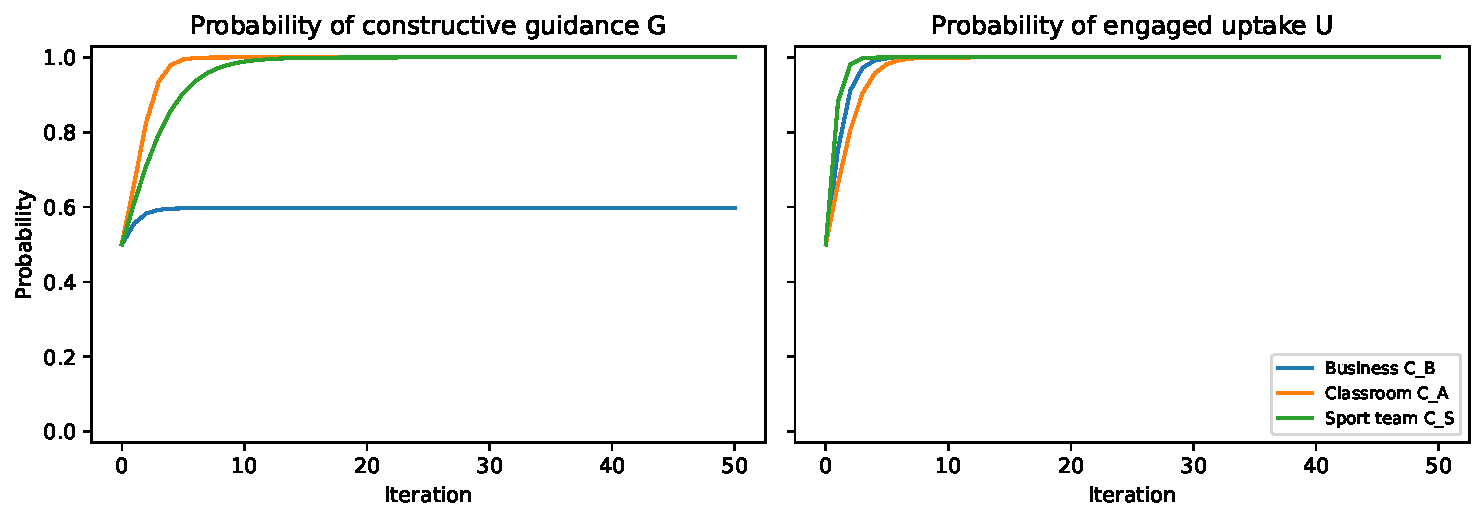
\includegraphics[width=0.96\textwidth]{strategy_trajectories.pdf}
\caption{\textbf{Benchmark strategy trajectories.} Discrete exponential-replicator trajectories for the benchmark contexts. Left: probability of constructive guidance $G$. Right: probability of engaged uptake $U$.}
\label{fig:strategy-trajectories}
\end{figure*}

\begin{figure*}[t]
\centering
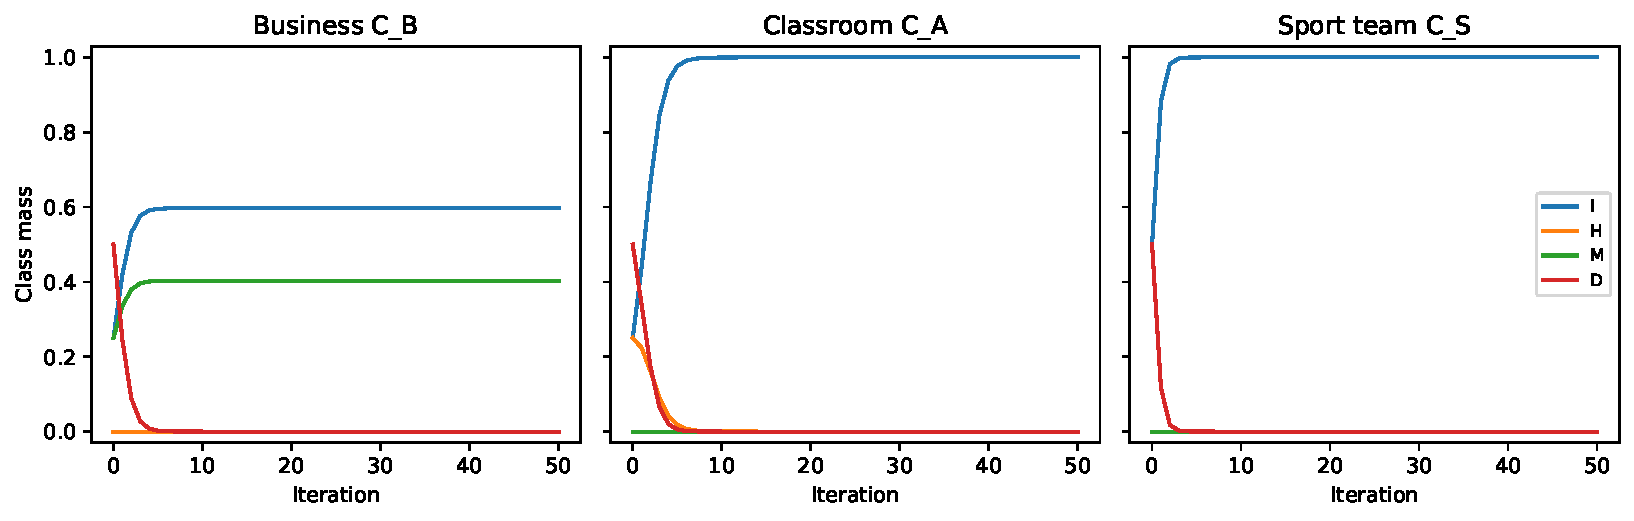
\includegraphics[width=0.98\textwidth]{class_masses.pdf}
\caption{\textbf{Induced class masses.} Class masses generated by the same exponential-replicator trajectories. The business context retains a positive malicious mass because $(P,U)$ remains strategically viable under engaged uptake.}
\label{fig:class-masses}
\end{figure*}

The simulation illustrates a point that is invisible in the static class table alone. The business context may converge to engaged uptake while retaining a positive mass on public pressure because public pressure and constructive guidance tie in the actor payoff against uptake. Hence some malicious class mass remains. In the classroom and sport contexts, the dynamics concentrate on constructive guidance and engaged uptake. This does not prove that real classrooms or sport teams behave this way; rather, it shows how contextual valuations can be used to generate testable population-level predictions once empirical calibration is available.

\begin{table*}[t]
\centering
\small
\begin{tabular}{lrrrrrr}
\toprule
Context & $p_{50}$ & $q_{50}$ & $E_{50}[W]$ & $\Pr_{50}(\Iclass)$ & $\Pr_{50}(\Mclass)$ & $\Pr_{50}(\Dclass)$\\
\midrule
Business $C_B$ & 0.597 & 1.000 & 2.985 & 0.597 & 0.403 & 0.000\\
Classroom $C_A$ & 1.000 & 1.000 & 5.000 & 1.000 & 0.000 & 0.000\\
Sport team $C_S$ & 1.000 & 1.000 & 6.000 & 1.000 & 0.000 & 0.000\\
\bottomrule
\end{tabular}
\caption{Final values for the illustrative run with $p_0=q_0=0.5$, $\eta=0.45$, and 50 iterations.}
\label{tab:simulation-final}
\end{table*}

\subsection{Fixed points, local stability, and the equilibrium knife-edge}
\label{sec:fixed-points}

The exponential-replicator update has enough structure to describe its fixed points and to explain why the business context behaves differently from the classroom and sport contexts. Write $p$ for the probability of $G$ and $q$ for the probability of $U$, and recall the expected actor-side payoffs
\begin{align*}
u_G(q)&=qX_C(G,U)+(1-q)X_C(G,R),\\
u_P(q)&=qX_C(P,U)+(1-q)X_C(P,R).
\end{align*}

\begin{proposition}[Invariant faces and benchmark fixed points]
\label{prop:fixed-points}
For every context $C$, each coordinate value in $\{0,1\}$ is invariant under the exponential-replicator map: if $p_t\in\{0,1\}$ then $p_{t+1}=p_t$, and likewise for $q$. Consequently the four vertices of $[0,1]^2$ are fixed points, including vertices that are not Nash equilibria, and $(G,U)$, i.e. $(p,q)=(1,1)$, is fixed in all three benchmark contexts. On the invariant edge $q=1$ the dynamics of $p$ are monotone and governed by the sign of
\[
u_G(1)-u_P(1)=X_C(G,U)-X_C(P,U).
\]
\end{proposition}

\begin{proof}
If $p_t=1$ the numerator and denominator of the $p$-update coincide, so $p_{t+1}=1$; if $p_t=0$ the numerator vanishes, so $p_{t+1}=0$. The same argument applies to $q$. Hence the edges $\{p\in\{0,1\}\}$ and $\{q\in\{0,1\}\}$ are invariant, and their four intersection points are fixed. At $q=1$ one has $u_G(1)=X_C(G,U)$ and $u_P(1)=X_C(P,U)$, and the exponential-replicator $p$-update satisfies $p_{t+1}>p_t$ when $u_G(1)>u_P(1)$, $p_{t+1}<p_t$ when $u_G(1)<u_P(1)$, and $p_{t+1}=p_t$ when $u_G(1)=u_P(1)$.
\end{proof}

The three benchmark contexts differ precisely in the actor-side selection gap along the uptake direction. A direct computation from Table~\ref{tab:payoff-transitions} gives
\[
u_G(q)-u_P(q)=
\begin{cases}
1-q, & \text{business } C_B,\\
3q, & \text{classroom } C_A,\\
1, & \text{sport } C_S.
\end{cases}
\]

\begin{proposition}[Strategic and dynamic non-robustness of the malicious phenomenon]
\label{prop:knife-edge}
In the business context the actor-side selection gap is $u_G(q)-u_P(q)=1-q$, which vanishes as $q\to1$. Consequently the segment $\{(p,1):p\in[0,1]\}$ is a continuum of fixed points, $(P,U)$ is a Nash equilibrium, and every interior initial condition leaves a strictly positive malicious mass $1-p_\infty>0$ in the limit. These properties use the exact actor indifference $X_{C_B}(G,U)=X_{C_B}(P,U)$. More precisely, hold all other business payoffs fixed and replace $X_{C_B}(G,U)=2$ by $2+\varepsilon$. If $\varepsilon>0$, the dynamics from every interior state converge to $(G,U)$ and malicious mass vanishes; if $\varepsilon<0$, they converge to $(P,U)$ and malicious mass tends to one. Thus arbitrarily small one-coordinate perturbations select opposite limiting equilibria. By contrast, in the classroom and sport contexts the actor gap equals $3q$ and $1$, which are positive near $q=1$, so $(G,U)$ attracts every interior trajectory and malicious mass vanishes.
\end{proposition}

\begin{proof}
The gap formulas follow by substituting the payoffs of Table~\ref{tab:payoff-transitions} into $u_G(q)-u_P(q)$. In the unperturbed business game the gap is $0$ at $q=1$, so every $p$ is fixed on that edge; it is exactly the continuum of mixed equilibria of Proposition~\ref{prop:mixed-equilibria}. For an interior start, the affected-side gap is $v_U(p)-v_R(p)=3p+1\ge1$, so the log odds of $q$ increase by at least $\eta$ per step and $1-q_t\to0$ geometrically. The cumulative actor drift $\sum_t\eta(1-q_t)$ is finite, hence the log odds of $p_t$ remain finite and $p_t\to p_\infty\in(0,1)$. Under the stated one-coordinate perturbation, the actor gap becomes $1-q+\varepsilon q$. The affected-side equation is unchanged, so $q_t\to1$. If $\varepsilon>0$, the actor gap is eventually bounded below by a positive constant and the log odds of $p_t$ diverge to $+\infty$, giving $p_t\to1$. If $\varepsilon<0$, the gap is eventually bounded above by a negative constant and the log odds diverge to $-\infty$, giving $p_t\to0$. In the classroom and sport contexts, $q_t\to1$ and the actor gaps $3q$ and $1$ are eventually bounded away from zero, so $p_t\to1$.
\end{proof}

This proposition isolates the conceptual core of the business benchmark. The \emph{class} of $(P,U)$ is robust: it remains malicious on an open region of weight and payoff space. Coexistence of the intelligent and malicious equilibria is not robust because it lies on the indifference hyperplane $X_{C_B}(G,U)=X_{C_B}(P,U)$. Class robustness and equilibrium robustness are therefore different requirements; the perturbation audit below quantifies this distinction without treating the synthetic draws as empirical data.

\subsection{Sensitivity to learning rate and initial conditions}

A single run is not sufficient to support even a minimal population-dynamics claim. We therefore report a deterministic sensitivity check over the wider grid
\[
\eta\in\{0.05,0.15,0.45,1.00,1.50\}
\]
and the five initial conditions
\[
\begin{gathered}
(p_0,q_0)\in\{(0.2,0.2),(0.2,0.8),(0.5,0.5),\\
(0.8,0.2),(0.8,0.8)\}.
\end{gathered}
\]
The resulting summary over 25 deterministic runs per context is shown in Table~\ref{tab:sweep}. The full grid is exported by the reproducibility notebook.

\begin{table*}[t]
\centering
\scriptsize
\resizebox{\textwidth}{!}{%
\begin{tabular}{ccccccc}
\toprule
Context & $p_{50}$ & $q_{50}$ & $E_{50}[W]$ & $\Pr_{50}(\Iclass)$ & $\Pr_{50}(\Mclass)$ & $\Pr_{50}(\Dclass)$\\
\midrule
Business $C_B$ & $[.223,.932]$ & $[.971,1]$ & $[1.094,4.661]$ & $[.222,.932]$ & $[.068,.775]$ & $[0,.029]$\\
Classroom $C_A$ & $[.942,1]$ & $[.918,1]$ & $[4.059,5]$ & $[.864,1]$ & $[0,0]$ & $[0,.058]$\\
Sport team $C_S$ & $[.753,1]$ & $[.9999,1]$ & $[5.505,6]$ & $[.9999,1]$ & $[0,0]$ & $[0,.0002]$\\
\bottomrule
\end{tabular}%
}
\caption{Ranges over the 25 deterministic design points formed by five learning rates and five initial conditions. These are design extrema, not sampling estimates or confidence intervals.}
\label{tab:sweep}
\end{table*}

The zero malicious mass in the classroom and sport rows follows from their class maps: neither game has a malicious profile. In the business game, public pressure remains payoff-equivalent to constructive guidance against uptake, so positive malicious mass persists at every design point. Its magnitude depends on the initial state and learning rate; the claim is viability under this constructed game, not a unique or empirically estimated mass.

\subsection{Computational robustness audits}

Four audits challenge the claims rather than merely regenerate the chosen
example.  The first enumerates all $2^8=256$ $2\times2$ sign-grid games with
payoffs in $\{-1,1\}$. Opponent-contingent strictly increasing zero-fixing
transformations preserve every
class map and every pure best-response correspondence.  Adding $2$ to each
payoff conditional on the opponent's action preserves every pure best response
but changes 255 of the 256 class maps, directly exercising
Theorem~\ref{thm:joint-preservation} and Corollary~\ref{cor:offset-separation}.

Second, we enumerate all $5^8=390{,}625$ $2\times2$ games whose eight payoff coordinates lie in $\{-2,-1,0,1,2\}$. Including zero admits boundary payoffs and additional weak best-response ties. Among these games there are 14,148 unordered pairs consisting of an intelligent and a malicious pure equilibrium. None shares the actor's action, 5,400 share the affected side's action with zero failures of the dominance conclusion in Theorem~\ref{thm:configuration}(b), and 8,748 share neither action. Of the last group, 1,372 consist of strict equilibria with the intelligent profile welfare-dominating the malicious profile.

Third, to test that the finite-game extension is not an artifact of square matrices, we enumerate every $2\times3$ and $3\times2$ game with payoff coordinates in $\{-2,-1,1\}$, or $2\cdot3^{12}=1{,}062{,}882$ rectangular games. The two negative levels allow a malicious profile to be a strict best response, while the larger $2\times2$ grid separately covers zero-payoff boundaries. The rectangular games contain 223,074 intelligent/malicious equilibrium pairs: zero share the actor's action, 100,602 share the affected side's action with zero dominance failures, and 122,472 share neither action. Among the last group, 5,184 pairs are strict and welfare ordered in the stated direction. These finite audits are not proofs, but they independently exercise rectangular best-response sets, search explicitly for counterexamples, and reproduce the theorem's three relative-position cases.

Finally, for each benchmark and each radius
\[
\delta\in\{0.25,0.50,0.75,0.99,1.01,1.50\},
\]
we draw 2,000 independent perturbation vectors uniformly from
$[-\delta,\delta]^8$ using the fixed seed 20260622. For every $\delta<1$, all
6,000 perturbed games preserve their benchmark class maps, as predicted by the
minimum axis margin. In the business game, however, none preserves the original
two-equilibrium set: a continuous perturbation breaks the actor tie with
probability one. Approximately half retain a malicious equilibrium alone,
depending on the sign of the broken tie. Figure~\ref{fig:payoff-perturbation}
contrasts class-map retention with equilibrium-set retention. The rates describe
the stated synthetic perturbation distribution; they are not inferential
estimates about real contexts.

\begin{figure*}[t]
\centering
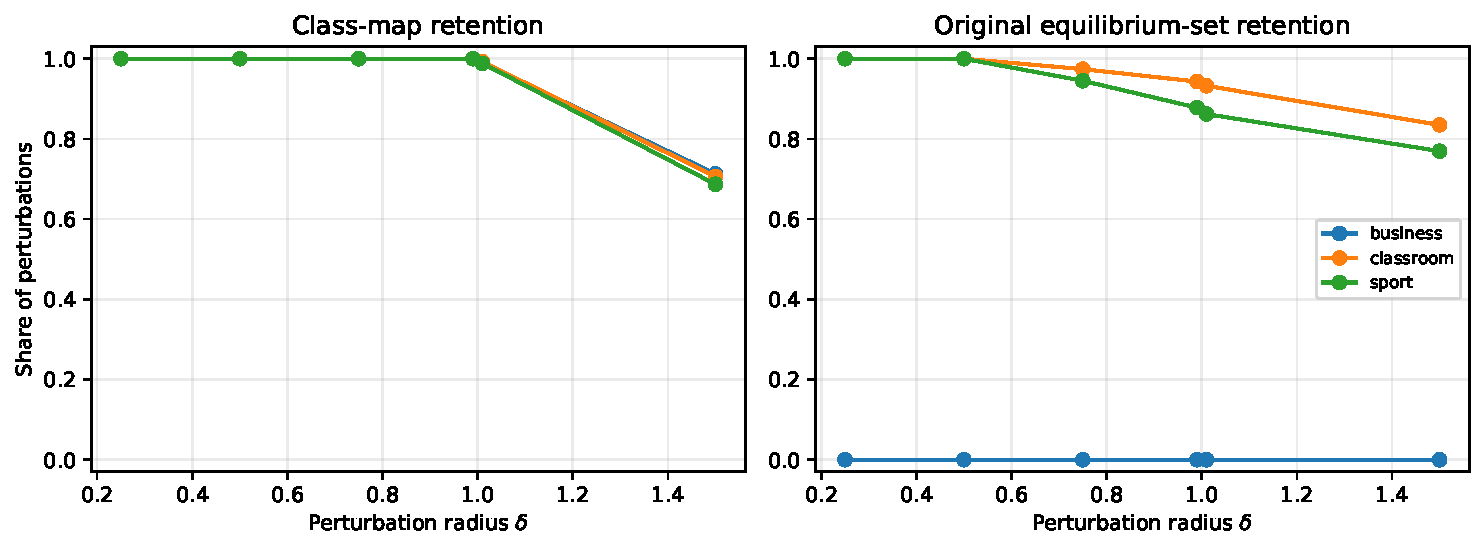
\includegraphics[width=0.90\textwidth]{payoff_perturbation_robustness.pdf}
\caption{\textbf{Payoff-perturbation robustness.} Retention rates under 2,000 seeded uniform payoff perturbations per context and radius. Class maps are locally robust, while the business benchmark's original equilibrium set is destroyed by every nonzero continuous perturbation because it requires an exact tie.}
\label{fig:payoff-perturbation}
\end{figure*}

\subsection{Connecting class sensitivity with dynamic distance}


The structural pseudometric $S$ compares contexts by class maps. A population model also yields trajectory distributions $\pi_t^C$ over profiles. For a fixed update rule $L$, horizon $T$, learning rate $\eta$, and initial condition $z_0=(p_0,q_0)$, define
\[
D_{\mathrm{traj}}^{L,T,\eta,z_0}(C,D)=\frac{1}{T+1}\sum_{t=0}^{T}\tfrac12\|\pi_t^C-\pi_t^D\|_1.
\]
The factor $\tfrac12$ makes each summand the total-variation distance between the two profile distributions, so $D_{\mathrm{traj}}\in[0,1]$ and is directly comparable with the structural class sensitivity $S(C,D)\in[0,1]$. When no ambiguity is possible, we write $D_{\mathrm{traj}}$. This notation emphasizes that the dynamic distance is not an intrinsic distance between contexts alone; it is relative to the chosen population process.

\begin{proposition}[Dynamic distance is process-dependent]
\label{prop:dtraj}
For fixed update rule $L$, horizon $T$, learning rate $\eta$, and initial condition $z_0$, $D_{\mathrm{traj}}^{L,T,\eta,z_0}$ is a pseudometric on the set of contexts with a common action structure. It depends on the induced trajectories and is not determined by the structural class sensitivity $S$ alone.
\end{proposition}

\begin{proof}
For each context $C$, the update rule determines a trajectory $(\pi_t^C)_{t=0}^T$ in the simplex over the common finite profile set. Nonnegativity and symmetry of $D_{\mathrm{traj}}^{L,T,\eta,z_0}$ follow from the corresponding properties of the $\ell^1$ norm. For the triangle inequality, for any contexts $C,D,E$ and each time $t$,
\[
\|\pi_t^C-\pi_t^E\|_1\le \|\pi_t^C-\pi_t^D\|_1+\|\pi_t^D-\pi_t^E\|_1.
\]
Multiplying by $\tfrac12$ and averaging this inequality over $t=0,\dots,T$ gives
\[
D_{\mathrm{traj}}^{L,T,\eta,z_0}(C,E)\le D_{\mathrm{traj}}^{L,T,\eta,z_0}(C,D)+D_{\mathrm{traj}}^{L,T,\eta,z_0}(D,E).
\]
Also $D_{\mathrm{traj}}^{L,T,\eta,z_0}(C,C)=0$. It is a pseudometric rather than a metric because distinct contexts can generate identical trajectories under a fixed update rule and initial condition.

The value of $D_{\mathrm{traj}}^{L,T,\eta,z_0}$ depends on the update rule, horizon, intensity, and initial condition because the trajectory $(\pi_t^C)$ does. It is not determined by $S$ alone: in the benchmark below, $S(C_B,C_A)=S(C_A,C_S)=2/4$, but Table~\ref{tab:traj-distance} gives very different dynamic distances for these pairs. Thus the structural and dynamic comparisons encode different information.
\end{proof}

For the benchmark run with $L$ equal to the exponential-replicator update, $\eta=0.45$, $p_0=q_0=0.5$, and $T=50$, we obtain Table~\ref{tab:traj-distance}.

\begin{table*}[t]
\centering
\small
\begin{tabular}{lccc}
\toprule
 & Business $C_B$ & Classroom $C_A$ & Sport team $C_S$\\
\midrule
Business $C_B$ & 0.000 & 0.385 & 0.373 \\
Classroom $C_A$ & 0.385 & 0.000 & 0.018 \\
Sport team $C_S$ & 0.373 & 0.018 & 0.000 \\
\bottomrule
\end{tabular}
\caption{Dynamic trajectory distance $D_{\mathrm{traj}}$ between contexts for the benchmark run, normalized as an averaged total-variation distance in $[0,1]$.}
\label{tab:traj-distance}
\end{table*}

The structural and dynamic distances are not the same object. Nevertheless, in this benchmark the classroom and sport contexts are dynamically close, even though their structural sensitivity is $S(C_A,C_S)=2/4$. The reason is that both dynamics concentrate rapidly on $(G,U)$. This illustrates why the paper distinguishes class structure from strategic and population behavior: contexts may differ in static classification but generate similar long-run behavior under a given learning rule.

\subsection{Reproducibility of numerical results}

The repository separates the model (\texttt{src/context\_games}), tests, experiments, notebook, and generated results. The notebook imports the tested package and is not a second implementation. The reproduction command first runs the unit and regression test suite, then regenerates all CSV tables and vector figures, and finally executes the source notebook to a separate artifact without modifying it. Continuous integration repeats the workflow under CPython 3.12.13 with a fully pinned environment.

The deterministic trajectories require no seed. Their horizon is checked at $T\in\{25,50,100,200,500\}$ using both the one-step residual and the change from the preceding horizon. At $T=50$ the maximum one-step residual over the three baseline contexts is $6.2\times10^{-11}$, and the largest change from $T=50$ to $T=100$ is $1.7\times10^{-10}$. The payoff-perturbation audit is stochastic only as a numerical integration over an explicitly specified synthetic distribution and uses the fixed seed 20260622. The exhaustive theorem audit is deterministic. All benchmark inputs, code, tests, and generated results are deposited with the article; no external or confidential data are used.

\FloatBarrier
\section{Methodological protocol for empirical calibration}
\label{sec:calibration}

Although the benchmark payoffs above are synthetic, the framework suggests a clear empirical route. A calibration study can proceed through contextual vignettes. A minimal pilot design would contain the following elements.

\begin{enumerate}[label=(\arabic*)]
\item \textbf{Profiles.} Select a family of abstract profiles, such as constructive guidance, public pressure, resistance, cooperative uptake, sanction, strategic sacrifice, and information withholding.
\item \textbf{Contextual instantiation.} Instantiate each profile in several contexts: organization, classroom, sport team, public institution, or family. Each vignette should identify the authority-side actor, the affected side, the action, and the response.
\item \textbf{Participants and estimands.} Define the target population, sampling frame, primary contrasts, exclusion rules, and smallest substantively relevant class-margin or context effect before recruitment. Determine sample size from a preregistered precision or power analysis that accounts for repeated judgments and clustering by participant and vignette; no universal pilot size is defensible.
\item \textbf{Measures.} Ask participants to estimate the gain or loss for the acting player and for the affected player on a scale from $-5$ to $5$. Additional items may measure perceived fairness, legitimacy, humiliation, learning, compliance, trust, or cohesion.
\item \textbf{Normalization.} Normalize responses into payoff vectors $(x,y)$ and compute induced benefit--loss classes.
\item \textbf{Uncertainty.} Use a hierarchical model or a cluster-respecting bootstrap to quantify uncertainty in both payoff coordinates. Report joint regions and the probability or confidence with which a profile lies on each side of an axis; marginal intervals alone do not identify quadrant membership.
\item \textbf{Hypotheses.} Preregister tests of context-by-profile contrasts, including whether profiles such as $(P,U)$ cross a specified axis and whether contextual sensitivity differs across domains. Correct for multiplicity or designate a single primary contrast.
\end{enumerate}

Such a study would test whether the theoretical phenomenon illustrated in Table~\ref{tab:payoff-transitions} appears in human judgments. It would also allow different communities to have different valuation maps without changing the abstract action structure. In such a study, the relevant empirical question is not whether a person is destructive, but whether a community evaluates a profile as producing non-compensating harm.

\FloatBarrier
\section{Discussion}
\label{sec:discussion}

The model developed here clarifies a distinction that is easily missed. An action structure describes who can do what. A contextual valuation describes what those actions mean in a given domain. The benefit--loss class is induced only after valuation. Therefore, class is neither purely strategic nor purely subjective. It is relational: it depends on the interaction between an abstract profile and a context-specific interpretation of gains and losses.

The partition-based formulation turns the original sign-plane intuition into a
comparative object. Each context induces a partition of the profile space, and
translations specify which profiles are treated as counterparts. More
importantly, Theorem~\ref{thm:joint-preservation} shows that preserving this
partition is not redundant with preserving pure incentives: payoff offsets can
be strategically invisible and semantically decisive.

The pseudometric $S$ provides a quantitative comparison of contexts at the class level. It ignores payoff magnitude and focuses on whether the induced relational class changes. This is appropriate when the question is not how much the payoffs change, but whether the social meaning of the interaction changes. The robustness theorem complements this by showing when class invariance is stable under perturbation: profiles far from the axes cannot be recontextualized by small valuation changes.

The game-theoretic layer adds a second distinction. An intelligent profile need not be a Nash equilibrium, and a malicious profile may be one. In the business benchmark, $(P,U)$ is malicious but admits no profitable unilateral deviation. In the sport benchmark, $(P,U)$ is intelligent but not an equilibrium. Thus class desirability and equilibrium membership should be studied jointly rather than conflated.

The population-dynamics illustration adds a third distinction. Static contextual sensitivity and dynamic trajectory distance need not agree. Two contexts may classify some profiles differently but converge to similar long-run behavior under a given update rule. Conversely, contexts with similar class maps may behave differently if the payoff magnitudes and ordinal comparisons induce different dynamics. This motivates later work connecting class-level metrics, equilibrium structure, and population dynamics more systematically.

\FloatBarrier
\section{Limitations and future work}
\label{sec:limitations}

The paper has several limitations. First, the numerical payoffs are constructed examples, not measurements of organizations, classrooms, or teams; robustness to perturbation does not confer external validity. Second, seven features encode four profiles, so the weight representation is saturated and non-identified. Third, the exponential-replicator illustration is deterministic, low-dimensional, and conditional on independent random matching. Its invariant faces make every pure vertex a rest point, including non-equilibria, and it contains neither mutation nor estimated behavioral noise. Fourth, the perturbation rates describe a chosen uniform distribution over synthetic payoffs and are computational diagnostics rather than sampling statements. Fifth, boundary cases require domain-specific conventions, especially when one player is neutral. Finally, the contextual valuation primitive and several partition observations are elementary and are not claimed as novel. The formal contribution is the comparative intersection of class and incentive preservation, together with the exact robustness and equilibrium-configuration results.

These limitations delimit the scope of the framework. Empirical calibration, probabilistic valuation, more parsimonious identified features, networked interaction, and alternative learning rules are natural next steps. Until such evidence exists, the domain labels should be read only as interpretations of synthetic games.

\section{Conclusion}
\label{sec:conclusion}

This paper developed a comparative framework for transporting Cipolla-style
benefit--loss classifications across contexts. It did not claim that
context-dependent utility is new. Its starting point is instead that the class
of a strategic profile is induced by a context-specific valuation and therefore
need not travel with the abstract profile.

The joint-preservation theorem identifies the exact
opponent-contingent separable transports that retain both classes and pure best
responses: strictly increasing transformations that fix zero. Its affine
corollary permits positive rescaling but excludes offsets. This establishes that social
classification contains information not recoverable from pure strategic
equivalence. Exact robustness radii then quantify how class maps and complete
pure-equilibrium sets can fail at different distances. The finite-game
configuration theorem separates an impossible shared-actor-action case, a
forced shared-affected-action knife-edge, and a potentially robust
no-shared-action regime. Exhaustive square and rectangular enumeration, seeded
perturbations, and convergence diagnostics challenge these claims
computationally.

The benchmark examples show how these notions operate in three domains: business organization, classroom, and sport team. The central transition $(P,U):\Mclass\to\Dclass\to\Iclass$ demonstrates that contextual valuation can move a profile from malicious, to destructive, to intelligent while leaving the abstract action structure unchanged. The second transition $(G,R):\Dclass\to\Hclass\to\Dclass$ shows that recontextualization is not always a movement toward improvement. This paper provides the structural and computational layer of that program: empirical calibration is not required for the validity of the formal results, but is the natural next step for domain-specific applications. Future work should estimate contextual valuations empirically, extend the framework to larger games and networks, and connect class transitions with dynamical models of trust, cohesion, performance, and accumulated harm.

\appendix
\section{Feature parameterization and weight-space robustness}
\label{sec:features}

The benchmark payoffs in Section~\ref{sec:benchmarks} are generated by a transparent feature-based parameterization. This appendix makes every numerical input inspectable and provides a template for later calibration, but it does not identify the weights empirically or make the synthetic payoffs non-arbitrary.

\begin{definition}[Feature-based valuation]
Let $\Prof=A\times B$ be a finite profile set. A feature representation is a map
\[
\phi:\Prof\to\R^k.
\]
A context-specific weight matrix is a matrix
\[
W_C\in\R^{2\times k}.
\]
The induced contextual valuation is
\[
V_C(\sigma)=W_C\phi(\sigma).
\]
The first row of $W_C$ determines the actor-side payoff, and the second row determines the affected-side payoff.
\end{definition}

The same feature vector may be evaluated differently in different contexts. For example, public pressure may increase short-term compliance in a business organization, damage pedagogical legitimacy in a classroom, and improve focus in a sport team when embedded in a shared competitive culture.

\begin{proposition}[Feature weights induce contextual revaluation]
Let $\phi:\Prof\to\R^k$ be fixed. If $W_C\ne W_D$, then the same profile $\sigma$ may satisfy
\[
Q(W_C\phi(\sigma))\ne Q(W_D\phi(\sigma)).
\]
\end{proposition}

\begin{proof}
It suffices to give an example. Let $k=1$, $\phi(\sigma)=1$, $W_C=(1,-1)^T$ and $W_D=(1,1)^T$. Then $W_C\phi(\sigma)=(1,-1)$ is malicious, while $W_D\phi(\sigma)=(1,1)$ is intelligent. Hence changing the context weights can change the class while the profile feature vector is fixed.
\end{proof}

For the benchmark examples we use two abstract strategies for the authority-side player:
\[
G=\text{constructive guidance},\qquad P=\text{public pressure},
\]
and two abstract strategies for the affected-side player:
\[
U=\text{engaged uptake},\qquad R=\text{resistance or withdrawal}.
\]
The symbol $U$ is used for uptake in order to avoid confusion with the destructive class $\Dclass$.

The feature vector is
\[
\phi(\sigma)=(g,p,u,r,pu,gr,pr)^T\in\R^7,
\]
where $g,p,u,r$ are indicators for guidance, pressure, uptake, and resistance, while $pu,gr,pr$ are interaction indicators for $(P,U)$, $(G,R)$, and $(P,R)$ respectively. Table~\ref{tab:feature-meaning} explains the features. Table~\ref{tab:features} gives the four feature vectors.

\begin{table}[h]
\centering
\small
\begin{tabular}{c p{0.74\textwidth}}
\toprule
Feature & Interpretation\\
\midrule
$g$ & Baseline effect of constructive guidance by the authority-side player.\\
$p$ & Baseline effect of public pressure by the authority-side player.\\
$u$ & Baseline effect of engaged uptake by the affected-side player.\\
$r$ & Baseline effect of resistance or withdrawal by the affected-side player.\\
$pu$ & Contextual interaction effect when public pressure is met with engaged uptake.\\
$gr$ & Contextual interaction effect when guidance is met with resistance.\\
$pr$ & Contextual interaction effect when pressure is met with resistance.\\
\bottomrule
\end{tabular}
\caption{Interpretation of the benchmark features. The weights assigned to these features encode context-specific norms, goals, and role expectations.}
\label{tab:feature-meaning}
\end{table}

\begin{table}[h]
\centering
\small
\begin{tabular}{cccccccc}
\toprule
Profile & $g$ & $p$ & $u$ & $r$ & $pu$ & $gr$ & $pr$\\
\midrule
$(G,U)$ & 1 & 0 & 1 & 0 & 0 & 0 & 0\\
$(G,R)$ & 1 & 0 & 0 & 1 & 0 & 1 & 0\\
$(P,U)$ & 0 & 1 & 1 & 0 & 1 & 0 & 0\\
$(P,R)$ & 0 & 1 & 0 & 1 & 0 & 0 & 1\\
\bottomrule
\end{tabular}
\caption{Feature representation for the four benchmark profiles.}
\label{tab:features}
\end{table}

\begin{table}[h]
\centering
\small
\begin{tabular}{llrrrrrrr}
\toprule
Context & Payoff row & $g$ & $p$ & $u$ & $r$ & $pu$ & $gr$ & $pr$\\
\midrule
$C_B$ business & actor & 1 & 0 & 1 & -2 & 1 & 0 & 0\\
 & affected & 1 & -1 & 2 & -2 & -3 & 0 & 0\\
\midrule
$C_A$ classroom & actor & 1 & -2 & 1 & -3 & 0 & 0 & 3\\
 & affected & 1 & -4 & 2 & 0 & 0 & 0 & 1\\
\midrule
$C_S$ sport team & actor & 2 & 1 & 1 & -3 & 0 & 0 & 0\\
 & affected & 1 & 0 & 2 & -2 & 0 & 0 & -1\\
\bottomrule
\end{tabular}
\caption{Context-specific weight matrices. Applying $V_C(\sigma)=W_C\phi(\sigma)$ generates the benchmark payoff matrices in Table~\ref{tab:payoff-transitions}.}
\label{tab:weights}
\end{table}

The weights in Table~\ref{tab:weights} are illustrative. Their signs encode the intended institutional readings: in the business benchmark, pressure can increase short-term actor-side control but reduce the affected side's autonomy and trust; in the classroom benchmark it is penalized on both sides; and in the sport benchmark it is positive only when combined with uptake. These statements define the examples and are not empirical claims about the three domains.

The representation is deliberately saturated relative to the four observed profiles: seven features generate only four payoff vectors per context, so the weight matrix is not identified from those vectors. Multiple weight matrices produce the same game. Accordingly, the feature layer is an auditable parameterization rather than an explanatory regression model. The formal robustness claims in this appendix concern sign-defined sets of payoffs or weights; empirical identification would require additional profiles, restrictions, or external data.


\begin{proposition}[Class regions in weight space]
\label{prop:weight-space-regions}
Fix a profile $\sigma$ and its feature vector $\phi(\sigma)\in\R^k$. For each open class $c\in\{\Iclass,\Hclass,\Mclass\}$, the set of weights $W\in\R^{2\times k}$ such that $Q(W\phi(\sigma))=c$ is an intersection of two strict linear half-spaces. The strict destructive region $\mathcal D^-$ is also an intersection of two strict linear half-spaces. Thus, away from $\mathcal D^0$ and the boundary, each class condition is stable under sufficiently small perturbations of $W$.
\end{proposition}

\begin{proof}
Write the two rows of $W$ as $w_1,w_2\in\R^k$. Then
\[
W\phi(\sigma)=\bigl(w_1\cdot\phi(\sigma),\, w_2\cdot\phi(\sigma)\bigr).
\]
For fixed $\phi(\sigma)$, the maps $W\mapsto w_1\cdot\phi(\sigma)$ and $W\mapsto w_2\cdot\phi(\sigma)$ are linear functions of the entries of $W$. The class conditions are therefore linear sign conditions on these two functions. Explicitly,
\[
Q(W\phi(\sigma))=\Iclass \Longleftrightarrow w_1\cdot\phi(\sigma)>0\text{ and }w_2\cdot\phi(\sigma)>0,
\]
\[
Q(W\phi(\sigma))=\Hclass \Longleftrightarrow w_1\cdot\phi(\sigma)<0\text{ and }w_2\cdot\phi(\sigma)>0,
\]
\[
Q(W\phi(\sigma))=\Mclass \Longleftrightarrow w_1\cdot\phi(\sigma)>0\text{ and }w_2\cdot\phi(\sigma)<0,
\]
and
\[
W\phi(\sigma)\in\mathcal D^- \Longleftrightarrow w_1\cdot\phi(\sigma)<0\text{ and }w_2\cdot\phi(\sigma)<0.
\]
Each condition is the intersection of two strict linear half-spaces in $\R^{2\times k}$. Strict linear half-spaces are open sets, and finite intersections of open sets are open. Hence if a weight matrix $W$ places $W\phi(\sigma)$ in one of these open classes, there exists a radius $\rho>0$ such that every weight matrix $W'$ with $\|W'-W\|<\rho$ induces the same class for $\sigma$. The exceptional cases are precisely those in which one of the two linear forms is zero, corresponding to $\mathcal D^0$ or to the boundary of the benefit--loss partition.
\end{proof}

This proposition addresses sensitivity, not empirical validity. The benchmark tables are one point in weight space, and nearby weights preserving the induced signs leave the class conclusions unchanged. This does not establish that the selected region describes any real institution.

\subsection{Robustness of benchmark transitions in weight space}

The next result is the main formal response to the concern that the benchmark payoffs are hand-crafted. It shows that the reported class transitions are not isolated numerical coincidences: they persist on open polyhedral regions of the weight space. Thus the exact entries in Table~\ref{tab:weights} are illustrative representatives of broader sign-defined parameter regions.

\begin{proposition}[Open weight conditions for the benchmark transitions]
\label{prop:benchmark-weight-conditions}
Let $\phi_{PU}=\phi(P,U)$ and $\phi_{GR}=\phi(G,R)$. Write the rows of the business, classroom, and sport-team weight matrices as
\[
W_B=(w_B^A,w_B^B),\qquad W_A=(w_A^A,w_A^B),\qquad W_S=(w_S^A,w_S^B),
\]
where the superscripts $A$ and $B$ denote actor-side and affected-side rows. Then the transition
\[
(P,U):\Mclass\longrightarrow\Dclass\longrightarrow\Iclass
\]
holds, with the classroom point in $\mathcal D^-$, if and only if
\[
w_B^A\cdot\phi_{PU}>0,\quad w_B^B\cdot\phi_{PU}<0,
\]
\[
w_A^A\cdot\phi_{PU}<0,\quad w_A^B\cdot\phi_{PU}<0,
\]
and
\[
w_S^A\cdot\phi_{PU}>0,\quad w_S^B\cdot\phi_{PU}>0.
\]
Similarly,
\[
(G,R):\Dclass\longrightarrow\Hclass\longrightarrow\Dclass
\]
with the destructive points in $\mathcal D^-$ holds if and only if
\[
w_B^A\cdot\phi_{GR}<0,\quad w_B^B\cdot\phi_{GR}<0,
\]
\[
w_A^A\cdot\phi_{GR}<0,\quad w_A^B\cdot\phi_{GR}>0,
\]
and
\[
w_S^A\cdot\phi_{GR}<0,\quad w_S^B\cdot\phi_{GR}<0.
\]
Each set of inequalities defines an open polyhedral region in the product of the three weight spaces.
\end{proposition}

\begin{proof}
For any context $C$, the class of a profile is determined by the signs of the two coordinates of $W_C\phi(\sigma)$, namely
\[
W_C\phi(\sigma)=\bigl(w_C^A\cdot\phi(\sigma),\, w_C^B\cdot\phi(\sigma)\bigr).
\]
For $(P,U)$ to be malicious in the business context, these two signs must be $(+,-)$, giving the first pair of inequalities. For $(P,U)$ to be strictly destructive in the classroom context, the signs must be $(-,-)$, giving the second pair. For $(P,U)$ to be intelligent in the sport-team context, the signs must be $(+,+)$, giving the third pair. This proves the first equivalence.

The proof for $(G,R)$ is identical. The transition $\Dclass\to\Hclass\to\Dclass$ with strict destructive endpoints requires signs $(-,-)$ in business, $(-,+)$ in classroom, and $(-,-)$ in sport. Translating these sign requirements into dot-product inequalities gives the displayed conditions.

Finally, each displayed condition is a strict linear inequality in the entries of the corresponding weight row. A finite conjunction of strict linear inequalities is an open polyhedral region. Therefore the benchmark transitions are not isolated numerical coincidences; they persist throughout open regions of the relevant weight spaces.
\end{proof}

The inequalities also identify which signs are substantively essential. For example, the transition $(P,U):\Mclass\to\Dclass\to\Iclass$ requires public pressure with uptake to be actor-beneficial and affected-side harmful in the business context, harmful to both sides in the classroom context, and beneficial to both sides in the sport-team context. If any of these sign requirements is reversed, the transition changes. The feature weights should therefore be read as a compact representation of institutional norms and role expectations rather than as empirical estimates.

\begin{table}[h]
\centering
\small
\begin{tabular}{ccccc}
\toprule
Profile & Business $C_B$ & Classroom $C_A$ & Sport team $C_S$ & Class transition\\
\midrule
$(P,U)$ & $(+,-)$ & $(-,-)$ & $(+,+)$ & $\Mclass\to\Dclass\to\Iclass$\\
$(G,R)$ & $(-,-)$ & $(-,+)$ & $(-,-)$ & $\Dclass\to\Hclass\to\Dclass$\\
\bottomrule
\end{tabular}
\caption{Essential sign patterns behind the two recontextualized benchmark profiles. The exact numerical payoffs in Table~\ref{tab:payoff-transitions} are representatives of these sign-defined regions.}
\label{tab:essential-signs}
\end{table}

\begin{table}[h]
\centering
\small
\setlength{\tabcolsep}{4pt}
\begin{tabular}{>{\raggedright\arraybackslash}p{0.19\textwidth}
                >{\centering\arraybackslash}p{0.12\textwidth}
                >{\raggedright\arraybackslash}p{0.60\textwidth}}
\toprule
Context & Sign of $(P,U)$ & Institutional reading of the essential signs\\
\midrule
Business $C_B$ & $(+,-)$ & Public pressure met with uptake raises the actor's short-term control but erodes the affected side's autonomy and trust.\\
Classroom $C_A$ & $(-,-)$ & Public pressure damages pedagogical legitimacy and student confidence, harming both sides.\\
Sport team $C_S$ & $(+,+)$ & Public pressure accepted as tactical discipline benefits both the actor and the team.\\
\bottomrule
\end{tabular}
\caption{Institutional reading of the essential sign conditions for the recontextualized profile $(P,U)$. It is the signs, not the exact magnitudes, that carry the social interpretation; this is exactly what Proposition~\ref{prop:benchmark-weight-conditions} formalizes.}
\label{tab:institutional-signs}
\end{table}

\FloatBarrier


\section*{Data and code availability}
All synthetic benchmark inputs, source code, tests, and scripts needed to reproduce the tables and figures are available at \url{https://github.com/cero1979/GamesAndContext}. The study uses no confidential or personal data. A versioned archival DOI will be added before submission.

\section*{Declaration of generative AI and AI-assisted technologies in the manuscript preparation process}
During revision, the author(s) used OpenAI Codex to assist with code refactoring, test construction, reproducibility checks, and language editing. The author(s) reviewed and edited all outputs, verified the mathematical and computational claims, and take full responsibility for the content of the article.

\begin{thebibliography}{99}

\bibitem[Arrow(1951)]{Arrow1951}
K. J. Arrow.
\emph{Social Choice and Individual Values}.
Wiley, 1951.

\bibitem[Ashlagi et al.(2008)]{AshlagiKrystaTennenholtz2008}
I. Ashlagi, P. Krysta, and M. Tennenholtz.
Social context games.
In \emph{Internet and Network Economics}, LNCS 5385, pages 675--683, 2008.
\url{https://doi.org/10.1007/978-3-540-92185-1_73}.

\bibitem[B\'{a}rcenas et al.(2020)]{Barcenas2020}
D. R. B\'{a}rcenas, J. Kuperman, and M. N. Kuperman.
The destructive effect of human stupidity: a revision of Cipolla's Fundamental Laws.
\emph{The European Physical Journal B}, 93:211, 2020.
\url{https://doi.org/10.1140/epjb/e2020-10339-3}.

\bibitem[Cipolla(2011)]{Cipolla2011}
C. M. Cipolla.
\emph{The Basic Laws of Human Stupidity}.
Il Mulino, Bologna, originally circulated in 1976; later editions, 2011.

\bibitem[Coleman(1990)]{Coleman1990}
J. S. Coleman.
\emph{Foundations of Social Theory}.
Harvard University Press, 1990.

\bibitem[Fehr and Schmidt(1999)]{FehrSchmidt1999}
E. Fehr and K. M. Schmidt.
A theory of fairness, competition, and cooperation.
\emph{Quarterly Journal of Economics}, 114(3):817--868, 1999.

\bibitem[Fishburn(1970)]{Fishburn1970}
P. C. Fishburn.
\emph{Utility Theory for Decision Making}.
Wiley, 1970.

\bibitem[Freund and Schapire(1999)]{FreundSchapire1999}
Y. Freund and R. E. Schapire.
Adaptive game playing using multiplicative weights.
\emph{Games and Economic Behavior}, 29(1--2):79--103, 1999.
\url{https://doi.org/10.1006/game.1999.0738}.

\bibitem[Gintis(2009)]{Gintis2009}
H. Gintis.
\emph{Game Theory Evolving: A Problem-Centered Introduction to Modeling Strategic Interaction}.
Princeton University Press, 2nd edition, 2009.

\bibitem[Hofbauer and Sigmund(1998)]{HofbauerSigmund1998}
J. Hofbauer and K. Sigmund.
\emph{Evolutionary Games and Population Dynamics}.
Cambridge University Press, 1998.

\bibitem[Jansen(1981)]{Jansen1981}
M. J. M. Jansen.
Regularity and stability of equilibrium points of bimatrix games.
\emph{Mathematics of Operations Research}, 6(4):530--550, 1981.
\url{https://doi.org/10.1287/moor.6.4.530}.

\bibitem[Kahneman and Tversky(1979)]{KahnemanTversky1979}
D. Kahneman and A. Tversky.
Prospect theory: an analysis of decision under risk.
\emph{Econometrica}, 47(2):263--291, 1979.

\bibitem[Kohlberg and Mertens(1986)]{KohlbergMertens1986}
E. Kohlberg and J.-F. Mertens.
On the strategic stability of equilibria.
\emph{Econometrica}, 54(5):1003--1037, 1986.
\url{https://doi.org/10.2307/1912320}.

\bibitem[Kuperman et al.(2020)]{Kuperman2020}
J. Kuperman, D. R. B\'{a}rcenas, and M. N. Kuperman.
Evolutionary game inspired by Cipolla's basic laws of human stupidity.
\emph{Physical Review E}, 101:052307, 2020.
\url{https://doi.org/10.1103/PhysRevE.101.052307}.

\bibitem[Mella(2017)]{Mella2017}
P. Mella.
Intelligence and stupidity: the educational power of Cipolla's test and of the Social Wheel.
\emph{Creative Education}, 8(15):2515--2534, 2017.

\bibitem[North(1990)]{North1990}
D. C. North.
\emph{Institutions, Institutional Change and Economic Performance}.
Cambridge University Press, 1990.

\bibitem[Osborne and Rubinstein(1994)]{OsborneRubinstein1994}
M. J. Osborne and A. Rubinstein.
\emph{A Course in Game Theory}.
MIT Press, 1994.

\bibitem[Ostrom(2005)]{Ostrom2005}
E. Ostrom.
\emph{Understanding Institutional Diversity}.
Princeton University Press, 2005.

\bibitem[Perissi and Bardi(2021)]{PerissiBardi2021}
I. Perissi and U. Bardi.
The Sixth Law of Stupidity: a biophysical interpretation of Carlo Cipolla's stupidity laws.
\emph{Systems}, 9(3):57, 2021.

\bibitem[Rabin(1993)]{Rabin1993}
M. Rabin.
Incorporating fairness into game theory and economics.
\emph{American Economic Review}, 83(5):1281--1302, 1993.

\bibitem[Rapoport et al.(1965)]{Rapoport1965}
A. Rapoport, A. M. Chammah, and C. J. Orwant.
\emph{Prisoner's Dilemma: A Study in Conflict and Cooperation}.
University of Michigan Press, 1965.

\bibitem[Ryan(2026)]{Ryan2026}
M. Ryan.
Category-dependent preferences and stochastic choice.
\emph{Mathematical Social Sciences}, 140:102514, 2026.
\url{https://doi.org/10.1016/j.mathsocsci.2026.102514}.

\bibitem[Sandholm(2010)]{Sandholm2010}
W. H. Sandholm.
\emph{Population Games and Evolutionary Dynamics}.
MIT Press, 2010.

\bibitem[Sen(1970)]{Sen1970}
A. Sen.
\emph{Collective Choice and Social Welfare}.
Holden-Day, 1970.

\bibitem[Su and Morsky(2024)]{SuMorsky2024}
R. Su and B. Morsky.
Relational utility and social norms in games.
\emph{Mathematical Social Sciences}, 127:54--61, 2024.
\url{https://doi.org/10.1016/j.mathsocsci.2023.12.001}.

\bibitem[Tettamanzi and da Pereira(2014)]{Tettamanzi2014}
A. G. B. Tettamanzi and C. C. da Pereira.
Testing Carlo Cipolla's laws of human stupidity with agent-based modeling.
In \emph{2014 IEEE/WIC/ACM International Joint Conferences on Web Intelligence and Intelligent Agent Technologies}, pages 246--253, 2014.

\bibitem[Tewolde and Conitzer(2024)]{TewoldeConitzer2024}
E. Tewolde and V. Conitzer.
Game transformations that preserve Nash equilibria or best-response sets.
In \emph{Proceedings of the Thirty-Third International Joint Conference on
Artificial Intelligence}, pages 2984--2993, 2024.
\url{https://doi.org/10.24963/ijcai.2024/331}.

\bibitem[Tversky and Kahneman(1981)]{TverskyKahneman1981}
A. Tversky and D. Kahneman.
The framing of decisions and the psychology of choice.
\emph{Science}, 211(4481):453--458, 1981.

\bibitem[Tversky and Simonson(1993)]{TverskySimonson1993}
A. Tversky and I. Simonson.
Context-dependent preferences.
\emph{Management Science}, 39(10):1179--1189, 1993.
\url{https://doi.org/10.1287/mnsc.39.10.1179}.

\bibitem[von Neumann and Morgenstern(1944)]{vonNeumann1944}
J. von Neumann and O. Morgenstern.
\emph{Theory of Games and Economic Behavior}.
Princeton University Press, 1944.

\bibitem[Weibull(1995)]{Weibull1995}
J. W. Weibull.
\emph{Evolutionary Game Theory}.
MIT Press, 1995.

\end{thebibliography}

\end{document}
